% ===========================================================================
%  LYRA — MANUALE UTENTE
% ===========================================================================
%
%  Il secondo documento del progetto, nella stessa cartella e con lo stesso
%  preambolo della guida dello sviluppatore. Condividere comune/ non è
%  un'economia: è ciò che fa sì che un riquadro «attenzione» abbia lo stesso
%  aspetto nei due documenti, e che chi passa dall'uno all'altro non debba
%  reimparare a leggere.
%
%  DIFFERENZE DALLA GUIDA, e sono deliberate:
%    - niente indice analitico (si consulta per schermata, non per termine);
%    - capitoli più corti, uno per area dell'applicazione;
%    - si parte sempre da ciò che si vede, non da come è fatto.
%
%  Compilazione:   make utente     (oppure: latexmk -pdf manuale-utente)
% ===========================================================================
\documentclass[11pt, a4paper, twoside, openany]{book}

% ===========================================================================
%  comune/preambolo.tex — impostazioni comuni ai due documenti
% ===========================================================================
%
%  Lo includono sia guida-sviluppatore.tex sia manuale-utente.tex. Ciò che
%  vale per uno solo dei due NON va qui: va nel suo file principale, altrimenti
%  fra sei mesi nessuno sa più perché una cosa è dove è.
%
%  Motore: pdfLaTeX. Non lualatex, non xelatex, e la scelta è deliberata —
%  questo preambolo usa solo pacchetti di una TeX Live di base, così chi riceve
%  la cartella compila senza installare nulla. Nessun font di sistema, nessun
%  --shell-escape, nessuna dipendenza da Python.
% ===========================================================================

% --- lingua e codifica ------------------------------------------------------
\usepackage[T1]{fontenc}
\usepackage[utf8]{inputenc}

%  L'italiano in due modi, perché non tutte le installazioni hanno il pacchetto
%  babel-italian (le immagini Docker di TeX Live «base» tipicamente no, e una
%  documentazione che non compila lì è inutile metà delle volte che serve).
%    - c'è italian.ldf  -> si usa quello, è la via normale;
%    - non c'è          -> babel >= 3.75 costruisce la lingua dal proprio file
%                          locale/it/babel-it.ini, che è sempre presente.
%  In entrambi i casi si ottengono «Capitolo», «Indice», «Figura», «Tabella».
%  La sillabazione italiana è un'altra cosa: sta nel FORMATO, non nel pacchetto,
%  e se manca si vede subito (parole spezzate all'inglese). Il controllo è in
%  fondo a questo file.
\IfFileExists{italian.ldf}
  {\usepackage[italian]{babel}}
  {\usepackage[italian, provide = *]{babel}}

\usepackage{csquotes}

% --- caratteri --------------------------------------------------------------
%  Palatino per il testo e per la matematica (mathpazo): la documentazione ha
%  formule — vol targeting, restringimento della covarianza — e un testo con la
%  matematica di un'altra famiglia si legge come due documenti incollati.
%  Helvetica ridotta per i titoli, monospazio di Latin Modern per il codice.
\usepackage{mathpazo}
\usepackage[scaled=0.90]{helvet}
\usepackage{lmodern}
\renewcommand{\ttdefault}{lmtt}

\usepackage{microtype}

% --- composizione del paragrafo ---------------------------------------------
%  Un documento pieno di nomi di file e di simboli in monospazio ha molte
%  parole che non si possono spezzare: `diagnose_regime_signals.py` e' lungo
%  quattro centimetri e non ha punti di sillabazione. Con i valori standard
%  TeX preferisce far sbordare la riga nel margine piuttosto che allargare
%  gli spazi, e il risultato si vede.
%
%  Questi tre valori invertono la preferenza: meglio una riga un po' larga di
%  spazi che una riga che esce dalla giustezza. `hbadness` alza la soglia di
%  segnalazione di conseguenza, cosi' il log continua a riportare i problemi
%  veri e non le righe lente che abbiamo appena autorizzato.
\tolerance = 1500
\emergencystretch = 3em
\hbadness = 2000

% --- impaginazione ----------------------------------------------------------
\usepackage[
  a4paper,
  inner = 28mm, outer = 24mm, top = 26mm, bottom = 28mm,
  headsep = 7mm, footskip = 12mm,
]{geometry}

\usepackage{emptypage}      % le pagine lasciate bianche restano davvero bianche

% Niente pagine bianche. I due documenti si leggono a schermo: la pagina
% vuota che il libro inserisce per far cominciare capitoli, parti e
% frontespizio sulla pagina di destra lì è solo un buco. Con l'opzione
% openany della classe i capitoli e le parti cominciano sulla pagina
% seguente; qui lo stesso vale per \frontmatter, \mainmatter e i
% \cleardoublepage scritti a mano (frontespizi), che la classe book
% eseguirebbe comunque. Il layout resta a due facciate (margini interno ed
% esterno, intestazioni alternate).
\let\cleardoublepage\clearpage
\usepackage{setspace}
\setstretch{1.06}

% --- colori, codice, figure -------------------------------------------------
\usepackage{etoolbox}
% ===========================================================================
%  comune/colori.tex — la tavolozza
% ===========================================================================
%
%  Sono i colori del PRODOTTO, non colori scelti per la documentazione: gli
%  stessi valori che stanno in dashboard/static/css/ui-v2.css e nella landing.
%  Documentare un prodotto con i colori di qualcun altro costringe chi legge a
%  tradurre due volte — una figura verde acqua qui e un pulsante verde acqua
%  nell'app sono la stessa cosa, e si deve vedere.
%
%  Chi cambia la tavolozza del prodotto cambia QUESTO file e nient'altro:
%  nessun altro file della documentazione nomina un colore per esteso.
% ===========================================================================
\RequirePackage{xcolor}

% --- i colori di base della landing -----------------------------------------
\definecolor{lyraInchiostro}{HTML}{111318}  % testo, titoli
\definecolor{lyraPannello}{HTML}{F5F5F2}    % fondo dei riquadri
\definecolor{lyraBordo}{HTML}{ECECEA}       % filetti e bordi
\definecolor{lyraAccento}{HTML}{2BB59A}     % verde acqua: l'unico accento
\definecolor{lyraPositivo}{HTML}{0F7A62}    % numeri in utile
\definecolor{lyraNegativo}{HTML}{9A3412}    % numeri in perdita

% --- i pastelli, usati per distinguere gli strati nelle figure --------------
\definecolor{lyraCielo}{HTML}{D9F1F7}
\definecolor{lyraMenta}{HTML}{DDF3E4}
\definecolor{lyraPesca}{HTML}{FFE4D4}
\definecolor{lyraLavanda}{HTML}{E6DEFF}
\definecolor{lyraCrema}{HTML}{FFF1C9}

% --- derivati, per bordi e testi sopra i pastelli ---------------------------
%  Si ricavano dai precedenti invece di essere scritti a mano: cambiando un
%  pastello, il suo bordo lo segue.
\colorlet{lyraCieloBordo}{lyraCielo!55!lyraInchiostro}
\colorlet{lyraMentaBordo}{lyraMenta!55!lyraInchiostro}
\colorlet{lyraPescaBordo}{lyraPesca!55!lyraInchiostro}
\colorlet{lyraLavandaBordo}{lyraLavanda!55!lyraInchiostro}
\colorlet{lyraCremaBordo}{lyraCrema!55!lyraInchiostro}

\colorlet{lyraGrigio}{lyraInchiostro!55}
\colorlet{lyraGrigioChiaro}{lyraInchiostro!28}
\colorlet{lyraAccentoScuro}{lyraAccento!70!lyraInchiostro}
\colorlet{lyraAccentoTenue}{lyraAccento!14!white}

% --- i colori del codice ----------------------------------------------------
\colorlet{codFondo}{lyraPannello}
\colorlet{codBordo}{lyraBordo}
\colorlet{codCommento}{lyraInchiostro!45}
\colorlet{codParola}{lyraAccentoScuro}
\colorlet{codStringa}{lyraNegativo!85}
\colorlet{codNumero}{lyraInchiostro!70}
\colorlet{codRiga}{lyraInchiostro!35}

% ===========================================================================
%  comune/stile-tikz.tex — il vocabolario grafico delle figure
% ===========================================================================
%
%  Ogni figura del progetto disegna con QUESTI stili e non con parametri
%  propri. La ragione e' leggibilita': se in una figura il riquadro di un
%  modulo e' azzurro e in quella dopo e' dello stesso azzurro un archivio su
%  disco, chi legge impara due volte e si fida zero. Qui un colore significa
%  una cosa sola in tutto il documento:
%
%     cielo     il MOTORE di calcolo (Python, core/)
%     menta     l'INTERFACCIA (Flask, dashboard/)
%     pesca     il SITO (Next.js) e tutto cio' che sta in rete
%     lavanda   i dati PERSISTENTI (disco, Postgres)
%     crema     cio' che viene da FUORI (broker, Stripe, provider dati)
%     bianco    strati astratti (porte, contratti, protocolli)
%
%  Questo file e' incluso sia dai documenti sia dalle figure compilate da sole
%  (figure/tikz/*.tex con la classe standalone), percio' non deve dipendere da
%  niente che esista solo dentro un documento.
% ===========================================================================
\RequirePackage{tikz}
\usetikzlibrary{
  arrows.meta, positioning, fit, backgrounds, calc, shapes.geometric,
  shapes.multipart, shapes.symbols, decorations.pathreplacing,
  decorations.pathmorphing, patterns, shadows.blur, matrix, chains, scopes
}

\tikzset{
  % --- impostazioni generali ----------------------------------------------
  every picture/.style = {
    line width = 0.7pt,
    font = \sffamily\small,
  },
  %
  % --- RIQUADRI: un modulo, un componente, una responsabilita' -------------
  riquadro/.style = {
    rectangle, rounded corners = 3pt, draw,
    minimum height = 9.5mm, minimum width = 30mm,
    inner xsep = 6pt, inner ysep = 5pt,
    align = center, font = \sffamily\small,
    text = lyraInchiostro,
  },
  motore/.style    = {riquadro, fill = lyraCielo,   draw = lyraCieloBordo},
  interfaccia/.style = {riquadro, fill = lyraMenta,  draw = lyraMentaBordo},
  sito/.style      = {riquadro, fill = lyraPesca,   draw = lyraPescaBordo},
  persistenza/.style = {riquadro, fill = lyraLavanda, draw = lyraLavandaBordo},
  esterno/.style   = {riquadro, fill = lyraCrema,   draw = lyraCremaBordo},
  astratto/.style  = {riquadro, fill = white, draw = lyraGrigio, dashed},
  %
  % Il riquadro piccolo: per gli elenchi fitti dove il nome basta.
  minuto/.style = {riquadro, minimum height = 7mm, minimum width = 22mm,
                   font = \sffamily\scriptsize, inner xsep = 4pt},
  %
  % --- FORME PARTICOLARI ---------------------------------------------------
  archivio/.style = {
    cylinder, shape border rotate = 90, aspect = 0.22, draw = lyraLavandaBordo,
    fill = lyraLavanda, minimum height = 13mm, minimum width = 22mm,
    inner xsep = 0pt, inner ysep = 4pt, align = center,
    font = \sffamily\scriptsize, text = lyraInchiostro,
  },
  decisione/.style = {
    diamond, draw = lyraInchiostro!60, fill = white, aspect = 1.9,
    inner xsep = 2pt, inner ysep = 0pt, align = center,
    font = \sffamily\scriptsize, text = lyraInchiostro,
  },
  persona/.style = {
    rectangle, rounded corners = 10pt, draw = lyraInchiostro!70,
    fill = white, minimum height = 9mm, minimum width = 24mm,
    align = center, font = \sffamily\small\itshape,
  },
  %
  % --- STRATI: il contenitore che raggruppa -------------------------------
  strato/.style = {
    rectangle, rounded corners = 5pt, draw = lyraGrigioChiaro,
    fill = lyraPannello!55!white, inner sep = 9pt,
  },
  stratoTitolo/.style = {
    font = \sffamily\scriptsize\bfseries, text = lyraInchiostro!65,
    anchor = north west,
  },
  %
  % --- FRECCE --------------------------------------------------------------
  %  Tre tipi, e la differenza va vista senza leggere la legenda:
  %    flusso      pieno    -> i dati passano di qui
  %    dipendenza  tratteg. -> questo conosce quello (ma nulla scorre)
  %    ritorno     grigio   -> la risposta che torna indietro
  flusso/.style = {
    -{Stealth[length = 2.4mm, width = 1.8mm]},
    draw = lyraInchiostro!75, line width = 0.8pt,
  },
  dipendenza/.style = {
    -{Stealth[length = 2.2mm, width = 1.6mm]}, dashed, dash pattern = on 2.4pt off 2pt,
    draw = lyraInchiostro!55, line width = 0.6pt,
  },
  ritorno/.style = {
    -{Stealth[length = 2.2mm, width = 1.6mm]},
    draw = lyraGrigio, line width = 0.6pt,
  },
  accento/.style = {
    -{Stealth[length = 2.6mm, width = 2mm]},
    draw = lyraAccento, line width = 1pt,
  },
  bloccato/.style = {
    -{Bar[width = 2.4mm]}, draw = lyraNegativo, line width = 0.9pt,
  },
  %
  % --- ETICHETTE SULLE FRECCE ---------------------------------------------
  etichetta/.style = {
    font = \sffamily\scriptsize, text = lyraInchiostro!70,
    fill = white, inner xsep = 2.5pt, inner ysep = 1pt,
  },
  etichettaAccento/.style = {etichetta, text = lyraAccentoScuro},
  %
  % --- NOTE A MARGINE ------------------------------------------------------
  nota/.style = {
    font = \sffamily\scriptsize\itshape, text = lyraInchiostro!60,
    align = left, inner sep = 2pt,
  },
  notaAccento/.style = {nota, text = lyraAccentoScuro, font = \sffamily\scriptsize},
  %
  % --- SEGNAPOSTO NUMERICI (1) (2) (3) sulle figure a passi ---------------
  passo/.style = {
    circle, draw = lyraAccento, fill = white, text = lyraAccentoScuro,
    font = \sffamily\scriptsize\bfseries, inner sep = 1.2pt,
    minimum size = 4.6mm,
  },
}

% --- la cornice con il titolo, usata dalle figure a strati -------------------
%  #1 opzioni  #2 nodi da contenere  #3 titolo
%  Il titolo sta SOPRA la cornice, non dentro: dentro finisce addosso al primo
%  nodo ogni volta che il nodo è vicino al bordo, e lo si scopre solo guardando
%  il PDF. Il nome del nodo è contato, così due strati nella stessa figura non
%  si sovrascrivono a vicenda.
\newcounter{lyrastratoN}
\newcommand{\lyrastrato}[3][]{%
  \stepcounter{lyrastratoN}%
  \begin{scope}[on background layer]
    \node[strato, fit = #2, #1] (cornice\thelyrastratoN) {};
    \node[stratoTitolo, anchor = south west]
      at ([shift={(1pt,1.5pt)}]cornice\thelyrastratoN.north west) {#3};
  \end{scope}}

% --- legenda compatta, da mettere sotto una figura ---------------------------
%  Si usa solo quando la figura introduce un colore nuovo: ripeterla sotto ogni
%  figura la fa diventare rumore che nessuno legge piu'.
\newcommand{\lyralegenda}[1]{%
  \begin{tikzpicture}[baseline]
    \matrix[matrix of nodes, nodes = {anchor = west, font = \sffamily\scriptsize},
            column sep = 3mm, row sep = 0.6mm] {#1\\};
  \end{tikzpicture}}

% ---------------------------------------------------------------------------
%  DUE TRAPPOLE, scritte qui perché costano mezz'ora ciascuna e l'errore che
%  producono indica sempre il punto sbagliato.
%
%  1. `\\` dentro un gruppo del contenuto di un nodo.
%        {testo\\{\scriptsize una riga\\e un'altra}}   <-- SI ROMPE
%        {testo\\{\scriptsize una riga}\\{\scriptsize e un'altra}}  <-- giusto
%     TikZ raccoglie le righe guardando i `\\` al primo livello: quello dentro
%     le graffe è il `\\` di LaTeX, che in un box orizzontale non ha senso.
%     L'errore che ne esce è «\tikzscope@linewidth non definito», segnalato sul
%     nodo DOPO quello colpevole.
%
%  2. Una tcolorbox dentro un nodo. Vale per \cod, \pulsante, \campo: sono
%     tcbox, cioè figure TikZ annidate, e lasciano la figura esterna in uno
%     stato incoerente. Stesso errore, stessa confusione. Nelle figure si usa
%     \codT (qui sotto).
% ---------------------------------------------------------------------------

% --- il codice DENTRO una figura --------------------------------------------
%  Nel testo un simbolo si scrive \cod{...}, che è un \tcbox: una tcolorbox,
%  cioè una tikzpicture. Infilarla dentro il contenuto di un nodo TikZ rompe lo
%  stato della figura che la contiene, e l'errore salta fuori sul nodo
%  SUCCESSIVO (`\tikzscope@linewidth` non definito) — mezz'ora buttata a
%  cercarlo nel posto sbagliato. Dentro le figure si usa questo, che è solo un
%  cambio di carattere e non apre niente.
%  \upshape serve davvero: dentro un nodo `nota`, che è in corsivo, un
%  monospazio corsivo si legge male e sembra un'altra cosa.
\newcommand{\codT}[1]{{\ttfamily\upshape\small\color{lyraInchiostro!85}#1}}

\newcommand{\lyravoce}[2]{%
  \tikz[baseline=-0.55ex]\node[#1, minimum width = 4.2mm, minimum height = 2.6mm,
        inner sep = 0pt, rounded corners = 1.4pt]{};~#2}

% ===========================================================================
%  comune/stile-codice.tex — come si mostra il codice
% ===========================================================================
%
%  PERCHE' listings E NON minted. minted colora meglio, ma per farlo chiama
%  Pygments durante la compilazione: serve Python installato e il permesso
%  --shell-escape, che molti editor LaTeX negano per difetto e che le
%  compilazioni automatiche rifiutano. Una documentazione che non compila sulla
%  macchina di chi la legge non e' documentazione. listings sta dentro LaTeX e
%  compila ovunque, e la differenza di resa non vale quel prezzo.
%
%  Tre modi di mostrare codice, e vanno usati per cose diverse:
%
%    \begin{codice}[python]{didascalia}{percorso/file.py}  blocco con cornice
%    \inputcodice{python}{didascalia}{file.tex}{percorso}  da file esterno
%    \cod{nome_simbolo}                                     dentro una frase
%
%  Il PERCORSO non e' decorazione: chi legge la documentazione ha il sorgente
%  aperto accanto, e un frammento senza il suo file costringe a cercarlo.
% ===========================================================================
\RequirePackage{listings}
\RequirePackage{tcolorbox}
\tcbuselibrary{listings, skins, breakable}

% --- stile comune ----------------------------------------------------------
\lstdefinestyle{lyraBase}{
  basicstyle      = \ttfamily\footnotesize\color{lyraInchiostro},
  keywordstyle    = \color{codParola}\bfseries,
  commentstyle    = \color{codCommento}\itshape,
  stringstyle     = \color{codStringa},
  numberstyle     = \ttfamily\scriptsize\color{codRiga},
  numbers         = left,
  numbersep       = 9pt,
  stepnumber      = 1,
  showstringspaces= false,
  breaklines      = true,
  breakatwhitespace = false,
  % La freccia dice che la riga continua: senza, una riga spezzata si legge
  % come due istruzioni, ed e' il tipo di errore che si propaga nel copia-incolla.
  prebreak        = \raisebox{0ex}[0ex][0ex]{\color{lyraAccento}\ensuremath{\hookleftarrow}},
  tabsize         = 4,
  columns         = fullflexible,
  keepspaces      = true,
  upquote         = true,
  extendedchars   = true,
  literate        =
    {à}{{\`a}}1 {è}{{\`e}}1 {é}{{\'e}}1 {ì}{{\`\i}}1 {ò}{{\`o}}1 {ù}{{\`u}}1
    {À}{{\`A}}1 {È}{{\`E}}1 {Ì}{{\`I}}1 {Ò}{{\`O}}1 {Ù}{{\`U}}1
    {€}{{\texteuro}}1 {°}{{\textdegree}}1 {·}{{\textperiodcentered}}1
    {—}{{---}}1 {–}{{--}}1 {«}{{\guillemotleft}}1 {»}{{\guillemotright}}1
    {“}{{\textquotedblleft}}1 {”}{{\textquotedblright}}1
    {’}{{\textquoteright}}1 {‘}{{\textquoteleft}}1
    {→}{{$\rightarrow$}}1 {←}{{$\leftarrow$}}1 {✓}{{$\checkmark$}}1,
}

% ---------------------------------------------------------------------------
%  REGOLA: dentro un blocco di codice si scrive SOLO ASCII.
%
%  Niente lettere accentate, niente caratteri di disegno, niente frecce.
%  `literate` non basta, e nemmeno il pacchetto listingsutf8: tcblisting
%  scrive il contenuto in un file intermedio e lo rilegge, quindi i byte
%  arrivano al kernel prima che listings possa intercettarli. L'errore e'
%  «Invalid UTF-8 byte sequence», segnalato nel file .listing e senza dire
%  quale blocco l'ha causato.
%
%  Quando un valore del sorgente contiene un accento, si translittera e si
%  mette un commento accanto. Gli alberi di cartelle si disegnano in ASCII
%  (|-- e `--), oppure in TikZ, dove non passano da listings.
%  `make controlla` segnala le violazioni prima che fermino la compilazione.
% ---------------------------------------------------------------------------

% --- i linguaggi che compaiono nel progetto ---------------------------------
\lstdefinelanguage{JavaScriptLyra}{
  keywords = {break, case, catch, class, const, continue, debugger, default,
    delete, do, else, export, extends, finally, for, function, if, import, in,
    instanceof, let, new, of, return, super, switch, this, throw, try, typeof,
    var, void, while, with, yield, async, await, static, get, set},
  keywordstyle = \color{codParola}\bfseries,
  ndkeywords = {true, false, null, undefined, document, window, console,
    fetch, JSON, Promise, Array, Object, Math},
  ndkeywordstyle = \color{lyraInchiostro!75}\bfseries,
  sensitive = true,
  comment = [l]{//},
  morecomment = [s]{/*}{*/},
  morestring = [b]',
  morestring = [b]",
  morestring = [b]`,
}

\lstdefinelanguage{TypeScriptLyra}{
  morekeywords = [1]{break, case, catch, class, const, continue, default,
    delete, do, else, enum, export, extends, finally, for, function, if,
    implements, import, in, instanceof, interface, let, new, of, private,
    protected, public, readonly, return, super, switch, this, throw, try,
    type, typeof, var, void, while, yield, async, await, as, satisfies},
  morekeywords = [2]{string, number, boolean, any, unknown, never, Promise,
    Record, Array, Partial, Required},
  keywordstyle = [1]\color{codParola}\bfseries,
  keywordstyle = [2]\color{lyraInchiostro!70},
  sensitive = true,
  comment = [l]{//},
  morecomment = [s]{/*}{*/},
  morestring = [b]',
  morestring = [b]",
  morestring = [b]`,
}

\lstdefinelanguage{Console}{
  basicstyle = \ttfamily\footnotesize,
  morecomment = [l]{\#},
  sensitive = false,
}

% --- l'ambiente principale --------------------------------------------------
%  #1 linguaggio, con il nome CORTO (python, js, ts, sql, json, yaml, html,
%     css, console): \lstlingua lo traduce nel nome che listings conosce, così
%     chi scrive non deve ricordare che JSON non esiste e che gli somiglia Java
%  #2 didascalia
%  #3 percorso del file nel progetto (vuoto = nessuno)
\newtcblisting{codiceInterno}[3]{
  listing only,
  % Sia lo stile sia la lingua devono stare QUI dentro: `listing options`
  % sostituisce `listing style` invece di aggiungersi, e il sintomo e' che
  % meta' delle impostazioni (breaklines, numeri di riga) sparisce senza
  % dirlo. Le righe lunghe escono dal riquadro, ed e' l'unico segno.
  listing options = {style = lyraBase, language = #1},
  breakable,
  enhanced,
  colback   = codFondo,
  colframe  = codBordo,
  boxrule   = 0.5pt,
  arc       = 3pt,
  left      = 3pt, right = 3pt, top = 4pt, bottom = 4pt,
  toptitle  = 2pt, bottomtitle = 2pt,
  title     = {\footnotesize\sffamily\bfseries\color{lyraInchiostro}#2%
               \ifstrempty{#3}{}{\hfill\normalfont\ttfamily\scriptsize
                 \color{lyraInchiostro!60}#3}},
  colbacktitle = lyraPannello!60!white,
  coltitle  = lyraInchiostro,
  fonttitle = \footnotesize,
  titlerule = 0pt,
  before skip = 10pt, after skip = 10pt,
}

% Nomi corti per i linguaggi, cosi' chi scrive non deve ricordare i nomi
% interni di listings ne' che JSON e YAML non esistono.
%
% Si usa \lstalias e non una macro che traduce: l'opzione `language` di
% listings viene letta senza espandere, quindi una macro li' dentro produce
% «Missing \endcsname» alla fine del blocco di codice — errore che non dice
% niente di cio' che e' successo.
\lstalias{console}{Console}
\lstalias{python}{Python}
\lstalias{js}{JavaScriptLyra}
\lstalias{ts}{TypeScriptLyra}
\lstalias{sql}{SQL}
\lstalias{json}{Java}      % JSON non esiste in listings: Java gli somiglia
\lstalias{yaml}{Python}    % idem per YAML: commenti con #, due punti, indentazione
\lstalias{html}{HTML}
\lstalias{css}{HTML}
\lstalias{testo}{}

% --- codice da file esterno -------------------------------------------------
%  #1 linguaggio  #2 didascalia  #3 percorso del file su disco  #4 percorso da
%  mostrare. Si usa per gli estratti lunghi tenuti fuori dal testo.
\newcommand{\inputcodice}[4]{%
  \begin{tcolorbox}[
    breakable, enhanced,
    colback = codFondo, colframe = codBordo, boxrule = 0.5pt, arc = 3pt,
    left = 3pt, right = 3pt, top = 4pt, bottom = 4pt,
    title = {\footnotesize\sffamily\bfseries\color{lyraInchiostro}#2%
             \hfill\normalfont\ttfamily\scriptsize\color{lyraInchiostro!60}#4},
    colbacktitle = lyraPannello!60!white, coltitle = lyraInchiostro,
    fonttitle = \footnotesize, titlerule = 0pt]
    \lstinputlisting[style=lyraBase, language=#1]{#3}
  \end{tcolorbox}}

% --- codice dentro una frase ------------------------------------------------
%  Fondo tenue invece del grassetto: dentro un paragrafo il grassetto chiama
%  l'occhio e spezza la lettura, mentre un nome di funzione va riconosciuto
%  senza essere gridato.
%  Le due penalita' attorno alla scatola non sono decorazione. Un \tcbox e'
%  una scatola indivisibile: se capita dopo una parentesi o un trattino --
%  cioe' senza spazio davanti -- TeX non ha dove spezzare la riga e la lascia
%  sbordare nel margine. Sono state la causa di quasi tutte le righe troppo
%  lunghe della prima stesura. Con queste, la scatola puo' sempre andare a
%  capo per conto suo.
%
%  Resta un limite: una scatola piu' larga della giustezza sborda comunque.
%  Per un percorso lungo si usa \file{} (testo normale, si spezza) oppure lo
%  si mette in un blocco di codice.
\DeclareRobustCommand{\cod}[1]{%
  \penalty50
  \tcbox[on line, boxsep = 0.6pt, left = 1.4pt, right = 1.4pt, top = 0pt,
         bottom = 0pt, arc = 2pt, boxrule = 0pt,
         colback = lyraPannello, colframe = lyraPannello]
        {\ttfamily\small #1}%
  \penalty0 }

% Percorso di file nel testo.
%  Usa lo stesso ciclo di \percorsoHTTP (definito in comune/macro.tex): un nome
%  come `diagnose_regime_signals.py' e' lungo quattro centimetri e senza punti
%  di sillabazione, quindi in una colonna stretta sborda. Con i punti di
%  interruzione dopo / _ . e - va a capo dove si legge comunque.
%  Il ciclo richiede ASCII e niente spazi: per il resto c'e' \cod{}.
\DeclareRobustCommand{\file}[1]{{\color{lyraInchiostro!78}\percorsoHTTP{#1}}}

% ===========================================================================
%  Un COMMENTO del sorgente citato per esteso
% ===========================================================================
%  Diversa da `codiceInterno`, e la differenza non e' estetica. Molti commenti
%  di questo progetto sono prose italiane di dieci righe che spiegano una
%  decisione: sono la parte piu' utile da citare, e dentro un blocco di
%  listings non ci stanno — listings vuole ASCII puro (vedi sopra), e
%  translitterare «perche'» e le lettere accentate significa citare qualcosa
%  che nel sorgente non c'e'.
%
%  Qui il testo e' testo LaTeX normale: accenti, virgolette e trattini lunghi
%  si compongono come nel resto del documento, e la citazione resta fedele.
%
%    \begin{commento}{percorso/del/file.py:120}
%    Il testo del commento, a capo come nel sorgente.
%    \end{commento}
%
%  Il corsivo e il filetto a sinistra dicono «questo l'ha scritto chi ha
%  scritto il codice, non chi ha scritto la guida».
\newtcolorbox{commento}[1]{
  enhanced, breakable,
  colback   = codFondo, colframe = lyraInchiostro!30,
  boxrule   = 0pt, leftrule = 2.2pt, arc = 2pt,
  left = 9pt, right = 9pt, top = 6pt, bottom = 6pt,
  fontupper = \small\itshape,
  title     = {\normalfont\ttfamily\scriptsize\color{lyraInchiostro!60}#1},
  colbacktitle = codFondo, coltitle = lyraInchiostro,
  titlerule = 0pt, toptitle = 2pt, bottomtitle = 0pt,
  before skip = 10pt, after skip = 10pt,
}


% --- numeri -----------------------------------------------------------------
%  In italiano il separatore delle migliaia sarebbe il punto, ma in un
%  documento pieno di valori numerici (soglie, quantili, prezzi) il punto
%  decimale inglese del codice e il punto delle migliaia del testo si
%  confondono. Spazio fine: non si confonde con niente.
\usepackage{siunitx}
\sisetup{group-separator = {\,}, group-minimum-digits = 4, detect-all}

% --- tabelle ----------------------------------------------------------------
\usepackage{booktabs}
\usepackage{longtable}
\usepackage{multirow}
\usepackage{array}
\usepackage{tabularx}
\usepackage{colortbl}

\newcolumntype{L}[1]{>{\raggedright\arraybackslash}p{#1}}
\newcolumntype{C}[1]{>{\centering\arraybackslash}p{#1}}
\newcolumntype{R}[1]{>{\raggedleft\arraybackslash}p{#1}}
\newcolumntype{M}{>{\ttfamily\footnotesize}l}

% Righe alternate tenui: su una tabella di venti righe l'occhio perde la riga,
% e un colore appena percepibile costa meno di una griglia piena.
\newcommand{\rigaTenue}{\rowcolor{lyraPannello!55!white}}

% --- elenchi ----------------------------------------------------------------
\usepackage{enumitem}
\setlist{itemsep = 1pt, parsep = 2pt, topsep = 4pt}
\setlist[itemize]{label = \textcolor{lyraAccento}{\textbullet}}
\setlist[enumerate]{label = \textcolor{lyraAccentoScuro}{\arabic*.}}

% --- figure -----------------------------------------------------------------
\usepackage{graphicx}
\usepackage{float}
\usepackage[font = small, labelfont = {bf, sf}, textfont = sf,
            labelsep = period, skip = 7pt]{caption}
\usepackage{subcaption}
\usepackage{adjustbox}
\graphicspath{{figure/}{figure/tikz/}{figure/schermate/}}

% --- intestazioni e piè di pagina -------------------------------------------
\usepackage{fancyhdr}
\usepackage{titlesec}
\usepackage{titletoc}

% --- riferimenti ------------------------------------------------------------
\usepackage[
  colorlinks = true,
  linkcolor  = lyraAccentoScuro,
  citecolor  = lyraAccentoScuro,
  urlcolor   = lyraAccentoScuro,
  filecolor  = lyraAccentoScuro,
  breaklinks = true,
  bookmarksnumbered = true,
  bookmarksopen = true,
  bookmarksopenlevel = 1,
]{hyperref}
\usepackage{url}
\urlstyle{sf}

% --- indice analitico -------------------------------------------------------
\usepackage{imakeidx}

% ===========================================================================
%  Stile dei titoli
% ===========================================================================
%  I capitoli si aprono con il numero grande a sinistra e un filetto verde
%  acqua: è il segno che si gira pagina in una sezione nuova, e lo si vede
%  sfogliando senza leggere.
\titleformat{\chapter}[display]
  {\sffamily\LARGE\bfseries\color{lyraInchiostro}}
  {\raggedright\normalfont\sffamily\fontsize{52}{52}\selectfont
   \color{lyraAccento!35!lyraPannello}\thechapter}
  {-6pt}
  {\raggedright}
  [\vspace{4pt}{\color{lyraAccento}\rule{\textwidth}{1.2pt}}]
\titlespacing*{\chapter}{0pt}{-24pt}{26pt}

\titleformat{\section}
  {\sffamily\large\bfseries\color{lyraInchiostro}}
  {\color{lyraAccentoScuro}\thesection}{0.7em}{}
\titlespacing*{\section}{0pt}{18pt}{7pt}

\titleformat{\subsection}
  {\sffamily\normalsize\bfseries\color{lyraInchiostro!88}}
  {\color{lyraAccentoScuro}\thesubsection}{0.6em}{}
\titlespacing*{\subsection}{0pt}{13pt}{4pt}

\titleformat{\subsubsection}[runin]
  {\sffamily\small\bfseries\color{lyraInchiostro!80}}
  {}{0pt}{}[\;---\;]
\titlespacing*{\subsubsection}{0pt}{9pt}{0.5em}

\setcounter{secnumdepth}{3}
\setcounter{tocdepth}{2}

% ===========================================================================
%  Indice
% ===========================================================================
%  L'indice è composto con titletoc, non con tocloft: i due pacchetti si
%  contendono le stesse macro e caricarli insieme rompe l'indice in modi che
%  si vedono solo a documento finito.
\titlecontents{chapter}[0pt]
  {\addvspace{9pt}\sffamily\bfseries}
  {\color{lyraAccentoScuro}\contentslabel{1.6em}}
  {}
  {\color{lyraInchiostro!55}\titlerule*[0.6pc]{.}\contentspage}
\titlecontents{section}[1.9em]
  {\sffamily\small}
  {\color{lyraInchiostro!70}\contentslabel{2.3em}}
  {}
  {\color{lyraInchiostro!45}\titlerule*[0.6pc]{.}\contentspage}

% ===========================================================================
%  I riquadri del testo
% ===========================================================================
%  Quattro soli, e ciascuno ha un lavoro preciso. Un documento con nove tipi di
%  riquadro è un documento in cui nessun riquadro significa qualcosa.
%
%    \begin{nota}{titolo}        un chiarimento utile, saltabile
%    \begin{attenzione}{titolo}  qui si rompe qualcosa
%    \begin{perche}{titolo}      perché è così e non altrimenti
%    \begin{pratica}{titolo}     cosa fare, passo per passo
% ===========================================================================
\newtcolorbox{nota}[1]{
  enhanced, breakable,
  colback = lyraCielo!35!white, colframe = lyraCieloBordo,
  boxrule = 0pt, leftrule = 2.2pt, arc = 2pt,
  left = 8pt, right = 8pt, top = 6pt, bottom = 6pt,
  fonttitle = \sffamily\bfseries\small,
  coltitle = lyraInchiostro,
  title = {#1}, titlerule = 0pt, colbacktitle = lyraCielo!35!white,
  toptitle = 1pt, bottomtitle = 1pt,
  before skip = 10pt, after skip = 10pt,
}

\newtcolorbox{attenzione}[1]{
  enhanced, breakable,
  colback = lyraPesca!40!white, colframe = lyraNegativo!70,
  boxrule = 0pt, leftrule = 2.2pt, arc = 2pt,
  left = 8pt, right = 8pt, top = 6pt, bottom = 6pt,
  fonttitle = \sffamily\bfseries\small,
  coltitle = lyraNegativo,
  title = {#1}, titlerule = 0pt, colbacktitle = lyraPesca!40!white,
  toptitle = 1pt, bottomtitle = 1pt,
  before skip = 10pt, after skip = 10pt,
}

\newtcolorbox{perche}[1]{
  enhanced, breakable,
  colback = lyraPannello, colframe = lyraGrigioChiaro,
  boxrule = 0pt, leftrule = 2.2pt, arc = 2pt,
  left = 8pt, right = 8pt, top = 6pt, bottom = 6pt,
  fonttitle = \sffamily\bfseries\small,
  coltitle = lyraInchiostro!75,
  title = {#1}, titlerule = 0pt, colbacktitle = lyraPannello,
  toptitle = 1pt, bottomtitle = 1pt,
  before skip = 10pt, after skip = 10pt,
}

\newtcolorbox{pratica}[1]{
  enhanced, breakable,
  colback = lyraMenta!45!white, colframe = lyraAccento,
  boxrule = 0pt, leftrule = 2.2pt, arc = 2pt,
  left = 8pt, right = 8pt, top = 6pt, bottom = 6pt,
  fonttitle = \sffamily\bfseries\small,
  coltitle = lyraAccentoScuro,
  title = {#1}, titlerule = 0pt, colbacktitle = lyraMenta!45!white,
  toptitle = 1pt, bottomtitle = 1pt,
  before skip = 10pt, after skip = 10pt,
}

% ===========================================================================
%  Macro del progetto
% ===========================================================================
% ===========================================================================
%  comune/macro.tex — le abbreviazioni del progetto
% ===========================================================================
%
%  Servono a scrivere una cosa in un posto solo. Il nome di un pacchetto
%  Python compare duecento volte nella guida: se un giorno `approaches/`
%  diventa `overlays/`, si cambia qui e non duecento volte a mano — e
%  soprattutto non si finisce con metà documento che dice una cosa e metà
%  un'altra, che è il modo in cui la documentazione smette di essere creduta.
% ===========================================================================

% --- la lingua del documento -----------------------------------------------
%  \iflyraInglese la definisce comune/preambolo.tex. Qui la si crea se manca,
%  perché `make figure' include questo file senza il preambolo. Il nome del
%  condizionale si scrive con \csname: scritto per esteso dentro un ramo
%  saltato, TeX lo conterebbe come un \if aperto e sbaglierebbe i \fi.
\ifcsname iflyraInglese\endcsname\else
  \expandafter\newif\csname iflyraInglese\endcsname
\fi

% --- nomi del prodotto ------------------------------------------------------
\newcommand{\Lyra}{\textsc{Lyra}}
\newcommand{\LyraCapital}{\textsc{Lyra Capital}}
\newcommand{\app}{\iflyraInglese the application\else l'applicazione\fi}
\newcommand{\App}{\iflyraInglese The application\else L'applicazione\fi}
\newcommand{\sito}{\iflyraInglese the site\else il sito\fi}
\newcommand{\Sito}{\iflyraInglese The site\else Il sito\fi}

% --- i pacchetti del motore -------------------------------------------------
%  Si scrivono \pkgCore e non \file{core/}: così il giorno in cui una cartella
%  cambia nome, cambia qui.
\DeclareRobustCommand{\pkg}[1]{{\ttfamily\small\color{lyraInchiostro!78}#1}}
\newcommand{\pkgCore}{\pkg{core/}}
\newcommand{\pkgStrategie}{\pkg{strategies/}}
\newcommand{\pkgApprocci}{\pkg{approaches/}}
\newcommand{\pkgPesi}{\pkg{weights/}}
\newcommand{\pkgOverlay}{\pkg{overlays/}}
\newcommand{\pkgRegime}{\pkg{regime/}}
\newcommand{\pkgDati}{\pkg{data/}}
\newcommand{\pkgBacktest}{\pkg{backtest/}}
\newcommand{\pkgLive}{\pkg{live/}}
\newcommand{\pkgEsecuzione}{\pkg{execution/}}
\newcommand{\pkgReport}{\pkg{reporting/}}
\newcommand{\pkgDashboard}{\pkg{dashboard/}}
\newcommand{\pkgDominio}{\pkg{domain/}}
\newcommand{\pkgPorte}{\pkg{ports/}}
\newcommand{\pkgApplicazione}{\pkg{application/}}
\newcommand{\pkgAdattatori}{\pkg{adapters/}}
\newcommand{\pkgComposizione}{\pkg{composition/}}
\newcommand{\pkgApi}{\pkg{api/}}

% --- termini del dominio, con la prima occorrenza indicizzata ---------------
\newcommand{\term}[1]{\emph{#1}\index{#1}}
\newcommand{\termdef}[1]{\textbf{#1}\index{#1}}

% --- riferimenti a classi, funzioni, file -----------------------------------
%  \simbolo{Nome}            una classe o una funzione
%  \sorgente{file.py}{120}   un punto preciso del sorgente
\DeclareRobustCommand{\simbolo}[1]{\cod{#1}}
\newcommand{\sorgente}[2]{{\ttfamily\footnotesize\color{lyraInchiostro!60}#1:#2}}

% --- tasti e voci dell'interfaccia, per il manuale utente -------------------
%  \voce{Overview}           una voce di menu o una scheda
%  \pulsante{Run backtest}   un pulsante da premere
%  \campo{Target vol}        un campo da compilare
%  \percorso{Settings > Data} un percorso di navigazione
\newcommand{\voce}[1]{\textsf{\textbf{#1}}}
\newcommand{\pulsante}[1]{%
  \tcbox[on line, boxsep = 1pt, left = 3pt, right = 3pt, top = 0.5pt,
         bottom = 0.5pt, arc = 3pt, boxrule = 0.5pt,
         colback = lyraInchiostro, colframe = lyraInchiostro,
         coltext = white]{\sffamily\scriptsize\bfseries #1}}
\newcommand{\pulsantesec}[1]{%
  \tcbox[on line, boxsep = 1pt, left = 3pt, right = 3pt, top = 0.5pt,
         bottom = 0.5pt, arc = 3pt, boxrule = 0.5pt,
         colback = white, colframe = lyraInchiostro!50,
         coltext = lyraInchiostro]{\sffamily\scriptsize\bfseries #1}}
\newcommand{\campo}[1]{\textsf{\itshape #1}}
\newcommand{\percorso}[1]{\textsf{\small #1}}
\newcommand{\freccia}{\;\textcolor{lyraAccento}{$\rightarrow$}\;}

% --- una rotta HTTP ---------------------------------------------------------
%  \rotta{GET}{/api/marketplace/<id>/perche-non-mio}
%
%  Esiste perche' \cod{} e' una scatola indivisibile: in una colonna di
%  tabella larga cinque centimetri un percorso lungo sborda, e non c'e'
%  niente che TeX possa fare. Qui il percorso e' testo normale e puo' andare
%  a capo dopo ogni barra, che e' il punto naturale.
%
%  Il ciclo prende un carattere alla volta: funziona perche' un percorso non
%  contiene spazi (un argomento non delimitato li mangerebbe) ed e' in ASCII
%  (una lettera accentata e' un carattere attivo e manda in errore il ciclo).
%  Per qualunque altra cosa si usa \cod{}.
\makeatletter
\def\lyra@finePercorso{\lyra@finePercorsoMARK}
\def\lyra@percorso#1{%
  \ifx#1\lyra@finePercorso
    \let\lyra@prossimo\relax
  \else
    #1%
    % Dopo questi quattro caratteri la riga puo' andare a capo. Sono i punti
    % in cui un percorso o un nome di file si leggono comunque bene spezzati.
    \ifx#1/\allowbreak\else
      \ifx#1\_\allowbreak\else
        \ifx#1.\allowbreak\else
          \ifx#1-\allowbreak\fi\fi\fi\fi
    \let\lyra@prossimo\lyra@percorso
  \fi
  \lyra@prossimo}
\DeclareRobustCommand{\percorsoHTTP}[1]{%
  {\ttfamily\small\color{lyraInchiostro!85}%
   \lyra@percorso#1\lyra@finePercorso}}
\makeatother

\DeclareRobustCommand{\rotta}[2]{%
  {\sffamily\scriptsize\bfseries\color{lyraAccentoScuro}#1}\,\percorsoHTTP{#2}}

% --- la figura standard -----------------------------------------------------
%  Centra, mette la didascalia sotto e l'etichetta. Esiste perché le tre righe
%  scritte a mano ogni volta divergono: una figura senza \label non si può
%  citare, e una citata per numero si rompe appena se ne aggiunge un'altra.
%  #1 file da includere (senza estensione)  #2 didascalia  #3 etichetta
%  `max width` e non `width`: una figura piccola resta della sua misura, una
%  piu' larga della giustezza viene rimpicciolita invece di sbordare nel
%  margine. Senza, ogni figura andrebbe dimensionata a mano e ridimensionata
%  a ogni modifica del testo.
\newcommand{\figuraTikz}[3]{%
  \begin{figure}[htbp]
    \centering
    \begin{adjustbox}{max width = \linewidth}
      \input{figure/tikz/#1}
    \end{adjustbox}
    \caption{#2}\label{fig:#3}
  \end{figure}}

%  Come sopra ma per un'immagine, con larghezza.
%  #1 larghezza  #2 file  #3 didascalia  #4 etichetta
\newcommand{\figuraImg}[4]{%
  \begin{figure}[htbp]
    \centering
    \includegraphics[width = #1\linewidth]{#2}
    \caption{#3}\label{fig:#4}
  \end{figure}}

%  Schermata con cornice: una schermata senza bordo si confonde con il fondo
%  della pagina, e non si capisce dove finisce l'interfaccia. La cornice sta
%  DENTRO la larghezza chiesta: altrimenti una schermata larga quanto la
%  pagina sborda di un punto per lato.
\newcommand{\figuraSchermata}[4]{%
  \begin{figure}[htbp]
    \centering
    \setlength{\fboxsep}{0pt}\setlength{\fboxrule}{0.5pt}%
    {\color{lyraGrigioChiaro}\fbox{\includegraphics[width = \dimexpr #1\linewidth - 2\fboxrule\relax]{#2}}}
    \caption{#3}\label{fig:#4}
  \end{figure}}

% --- riferimenti incrociati con la parola davanti ---------------------------
%  In inglese la parola vuole la maiuscola («see Chapter 4»), in italiano no.
\newcommand{\vediFig}[1]{\iflyraInglese Figure\else figura\fi~\ref{fig:#1}}
\newcommand{\vediTab}[1]{\iflyraInglese Table\else tabella\fi~\ref{tab:#1}}
\newcommand{\vediCap}[1]{\iflyraInglese Chapter\else capitolo\fi~\ref{cap:#1}}
\newcommand{\vediSez}[1]{\iflyraInglese Section~\else \S\,\fi\ref{sez:#1}}

% --- numeri e unità ---------------------------------------------------------
%  Ogni lingua con la sua convenzione, la stessa dell'applicazione e del sito:
%  in italiano «10\,%» e «49\,€», in inglese «10%» e «€49» (le migliaia, in
%  inglese, si scrivono con la virgola nell'argomento: \eur{1,490}).
\newcommand{\perc}[1]{\iflyraInglese #1\%\else #1\,\%\fi}
\newcommand{\eur}[1]{\iflyraInglese \texteuro#1\else #1\,\texteuro\fi}


% ===========================================================================
%  Le macro dentro i segnalibri del PDF
% ===========================================================================
%  hyperref deve trasformare il titolo di ogni capitolo e sezione in una
%  stringa semplice per il pannello dei segnalibri. Le macro che compongono
%  qualcosa — una scatola colorata, un ciclo sui caratteri — lo mandano in
%  tilt: l'errore e' «TeX capacity exceeded [input stack size]» su una riga
%  che non ha niente di strano, tipo
%      \subsection{Che cosa c'e' sotto \file{data/}}
%
%  Qui si dice a hyperref di considerarle, nei soli segnalibri, come
%  «stampa il contenuto e basta».
\pdfstringdefDisableCommands{%
  \makeatletter
  \let\file\@firstofone
  \let\cod\@firstofone
  \let\pkg\@firstofone
  \let\simbolo\@firstofone
  \let\percorsoHTTP\@firstofone
  \let\voce\@firstofone
  \let\campo\@firstofone
  \let\pulsante\@firstofone
  \let\pulsantesec\@firstofone
  \let\percorso\@firstofone
  \let\term\@firstofone
  \let\termdef\@firstofone
  \def\rotta#1#2{#1 #2}%
  \def\freccia{ > }%
  \def\Lyra{Lyra}%
  \def\LyraCapital{Lyra Capital}%
  \makeatother
}

% ===========================================================================
%  Controllo: la sillabazione italiana c'è davvero?
% ===========================================================================
%  I pattern di sillabazione si caricano quando si GENERA il formato, non
%  quando si compila: se mancano, babel non fallisce — ripiega sull'inglese, e
%  il documento esce con le parole spezzate nei punti sbagliati. È un difetto
%  che si vede solo guardando la pagina, quindi vale la pena dirlo nel log.
%
%  Per rimediare, su una TeX Live completa: `tlmgr install hyphen-italian`;
%  su Debian/Ubuntu: `apt install texlive-lang-italian`; poi `fmtutil-sys
%  --byfmt pdflatex`.
%
%  Il controllo guarda \language, che è un parametro intero del motore e si
%  può sempre confrontare: 0 è la lingua di partenza (inglese). Se dopo aver
%  selezionato l'italiano siamo ancora lì, i pattern non ci sono.
\AtBeginDocument{%
  \ifnum\language = 0
    \PackageWarningNoLine{lyra}{%
      Pattern di sillabazione ITALIANI assenti: il testo sara' spezzato\MessageBreak
      con le regole inglesi. Installare hyphen-italian e rigenerare il\MessageBreak
      formato (fmtutil-sys --byfmt pdflatex)}%
  \fi}


\hypersetup{
  pdftitle  = {Lyra — Manuale utente},
  pdfauthor = {Lyra Capital},
  pdfsubject = {Guida all'uso dell'applicazione},
  pdfkeywords = {Lyra, manuale, strategie, backtest, live, community, marketplace},
}

% --- intestazioni -----------------------------------------------------------
\pagestyle{fancy}
\fancyhf{}
\renewcommand{\headrulewidth}{0pt}
\renewcommand{\chaptermark}[1]{\markboth{\thechapter.\ #1}{}}
\renewcommand{\sectionmark}[1]{\markright{\thesection\ #1}}
\fancyhead[LE]{\sffamily\scriptsize\color{lyraInchiostro!55}\leftmark}
\fancyhead[RO]{\sffamily\scriptsize\color{lyraInchiostro!55}\rightmark}
\fancyfoot[LE,RO]{\sffamily\small\color{lyraInchiostro!70}\thepage}
\fancyfoot[RE,LO]{\sffamily\scriptsize\color{lyraInchiostro!40}Lyra · Manuale utente}

\fancypagestyle{plain}{%
  \fancyhf{}%
  \renewcommand{\headrulewidth}{0pt}%
  \fancyfoot[LE,RO]{\sffamily\small\color{lyraInchiostro!70}\thepage}%
  \fancyfoot[RE,LO]{\sffamily\scriptsize\color{lyraInchiostro!40}Lyra · Manuale utente}}

\begin{document}

\frontmatter
% ===========================================================================
%  comune/frontespizio-utente.tex
% ===========================================================================
\begin{titlepage}
\thispagestyle{empty}
\begin{tikzpicture}[remember picture, overlay]

  \fill[lyraInchiostro] (current page.north west)
    rectangle ([yshift = -9mm]current page.north east);

  \node[anchor = north west, inner sep = 0pt]
    at ([shift = {(28mm, -42mm)}]current page.north west)
    {\begin{minipage}{125mm}
       {\sffamily\fontsize{10}{12}\selectfont
        \color{lyraAccentoScuro}\bfseries
        LYRA CAPITAL\par}
       \vspace{3mm}
       {\sffamily\fontsize{40}{44}\selectfont\color{lyraInchiostro}
        Manuale\\utente\par}
       \vspace{5mm}
       {\color{lyraAccento}\rule{34mm}{1.6pt}\par}
       \vspace{6mm}
       {\sffamily\fontsize{12}{17}\selectfont\color{lyraInchiostro!62}
        Che cosa fa ogni schermata, in quale ordine\\
        si usano, e che cosa significano i numeri.\par}
     \end{minipage}};

  \node[anchor = south west, inner sep = 0pt]
    at ([shift = {(28mm, 34mm)}]current page.south west)
    {\begin{minipage}{125mm}
       \begin{tcolorbox}[enhanced, colback = lyraPannello,
                         colframe = lyraBordo, boxrule = 0.6pt, arc = 4pt,
                         left = 10pt, right = 10pt, top = 9pt, bottom = 9pt]
         {\sffamily\footnotesize\color{lyraInchiostro}%
          \textbf{Come si legge.} Ogni capitolo è una zona dell'applicazione.
          Si può leggere dall'inizio, oppure aprire direttamente il capitolo
          della schermata che si ha davanti.\par
          \vspace{4pt}
          \textbf{Per modificare Lyra}, non per usarla, il documento è un
          altro: la \emph{Guida dello sviluppatore}, nella stessa cartella.\par}
       \end{tcolorbox}
     \end{minipage}};

  \node[anchor = south east, inner sep = 0pt, align = right]
    at ([shift = {(-24mm, 18mm)}]current page.south east)
    {\sffamily\scriptsize\color{lyraInchiostro!45}
     Documento generato da sorgente \LaTeX\\
     \today};

\end{tikzpicture}
\end{titlepage}

\cleardoublepage

\thispagestyle{empty}
\vspace*{18mm}

{\sffamily\Large\bfseries\color{lyraInchiostro}Prima di cominciare\par}
\vspace{3mm}
{\color{lyraAccento}\rule{\textwidth}{1pt}\par}
\vspace{7mm}

\noindent
Lyra serve a costruire strategie di investimento, provarle sui dati del
passato e — quando reggono — farle girare su un conto vero. Le tre cose si
fanno in quest'ordine, e il manuale segue lo stesso ordine.

\vspace{4mm}
\noindent
Nel testo, \voce{Questa} è una voce di menu o una scheda, \pulsante{Questo} un
pulsante da premere, \campo{questo} un campo da compilare, e
\percorso{Settings \freccia Data} significa: apri \voce{Settings}, poi la
scheda \voce{Data}.

\vspace{6mm}
{\sffamily\large\bfseries\color{lyraInchiostro}I riquadri\par}
\vspace{3mm}

\begin{nota}{Nota}
Un chiarimento. Saltandolo, l'operazione riesce lo stesso.
\end{nota}

\begin{pratica}{In pratica}
L'operazione, passo per passo.
\end{pratica}

\begin{attenzione}{Attenzione}
Qui si perde qualcosa: dati, denaro, o tempo. Vale la pena leggerlo prima.
\end{attenzione}

\vspace{6mm}
\begin{perche}{Una parola sui numeri}
Nessun risultato mostrato dall'applicazione è una previsione. Un backtest dice
come una strategia si \emph{sarebbe} comportata sui dati del passato, con i
costi stimati; non dice come si comporterà. Il capitolo sugli \voce{Streams}
spiega quali numeri guardare per distinguere una strategia che ha funzionato
da una che ha avuto fortuna.
\end{perche}

\cleardoublepage


\tableofcontents

\mainmatter

% ===========================================================================
%  utente/01-primi-passi/00-capitolo.tex
% ===========================================================================
\chapter{Primi passi}\label{cap:primi-passi}

\begin{attenzione}{I numeri nelle schermate sono inventati}
Tutte le immagini di questo manuale sono state fatte su un'installazione con
\emph{dati di esempio}: serie generate al calcolatore, non prezzi reali e non
risultati di strategie. Servono a mostrare dove si trovano le cose. Nessuno
Sharpe, nessun rendimento e nessun drawdown di queste pagine significa
qualcosa.
\end{attenzione}

\section{Che cosa fa Lyra}\label{sez:cosa-fa}

Tre cose, in quest'ordine:

\begin{enumerate}
  \item \textbf{Costruire} una strategia di investimento --- scrivendola,
        disegnandola a blocchi, o descrivendola a parole.
  \item \textbf{Provarla} sui dati del passato, con i costi, e vedere come si
        sarebbe comportata.
  \item \textbf{Farla girare} su un conto vero, quando regge.
\end{enumerate}

\noindent
Le strategie si possono anche combinare fra loro, e si possono comprare e
vendere fra utenti nel \voce{Marketplace}. Questo manuale segue lo stesso
ordine: un capitolo per zona dell'applicazione.

\figuraTikz{flusso-utente}
  {Le zone dell'applicazione, nell'ordine in cui si usano. La freccia che
   torna indietro è la parte più frequente del lavoro.}
  {flusso-utente}

\section{Il menu}\label{sez:menu}

La barra a sinistra è sempre presente. Si allarga passandoci sopra con il
mouse e mostra i nomi delle voci.

\begin{figure}[htbp]
  \centering
  \setlength{\fboxsep}{0pt}\setlength{\fboxrule}{0.5pt}%
  {\color{lyraGrigioChiaro}\fbox{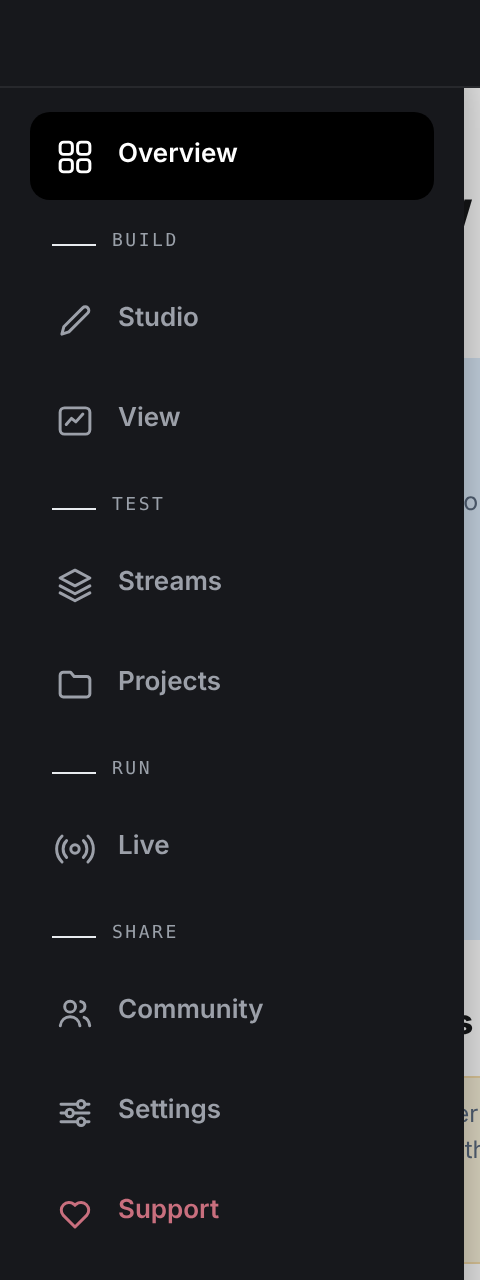
\includegraphics[width = 0.26\linewidth]
    {figure/schermate/menu.png}}}
  \caption{Il menu, allargato. Le voci sono in quattro gruppi: costruire,
           provare, far girare, comunità.}
  \label{fig:menu}
\end{figure}

\begin{center}
\begin{tabular}{@{}L{26mm}L{18mm}L{90mm}@{}}
\toprule
\textbf{Voce} & \textbf{Gruppo} & \textbf{A che serve} \\
\midrule
\rigaTenue
\voce{Overview} & Workspace & La schermata iniziale: come va tutto, in una
  pagina. \\
\voce{Studio} & Build & Dove si costruiscono le strategie. \\
\rigaTenue
\voce{View} & Build & I grafici con sopra quello che la strategia ha fatto. \\
\voce{Streams} & Test & I risultati: una scheda per strategia. \\
\rigaTenue
\voce{Projects} & Test & Le combinazioni di più strategie. \\
\voce{Live} & Run & Il collegamento a un conto vero. \\
\rigaTenue
\voce{Marketplace} & Community & Comprare e vendere strategie. \\
\voce{Settings} & Settings & Dati, parametri, regimi di mercato. \\
\bottomrule
\end{tabular}
\end{center}

\begin{nota}{In alto a destra}
La lente cerca in tutta l'applicazione; la campanella mostra i lavori
conclusi e i messaggi; il sole cambia fra chiaro e scuro; l'ultima voce è
l'accesso al proprio conto.
\end{nota}

\section{Serve un account?}\label{sez:account-serve}

Per costruire, provare e far girare le strategie, \textbf{no}:
l'applicazione gira sul computer di chi la usa e non chiede nulla.

Serve un account solo per le zone che passano dalla rete: il
\voce{Marketplace}, i messaggi, il profilo, l'abbonamento. Aprendo una di
quelle senza aver fatto l'accesso, l'applicazione lo dice e offre di farlo.

\section{L'ordine in cui si lavora}\label{sez:ordine}

\begin{pratica}{Dal nulla al primo risultato}
\begin{enumerate}
  \item \percorso{Settings \freccia Data}: scaricare i dati. Senza, tutte le
        pagine sono vuote --- non è un errore, non c'è niente da mostrare.
  \item \percorso{Streams \freccia Run backtest}: scegliere una strategia e
        premere \pulsante{Run backtest}.
  \item Aspettare. Il lavoro gira in sottofondo e la campanella avvisa alla
        fine; nel frattempo si può usare il resto dell'applicazione.
  \item \voce{Streams}: il risultato è comparso come scheda.
  \item \voce{Projects}: combinare due o più risultati.
  \item \voce{Live}: collegare un broker, quando si è pronti.
\end{enumerate}
\end{pratica}

% ===========================================================================
%  utente/02-overview/00-capitolo.tex
% ===========================================================================
\chapter{Overview}\label{cap:overview}

È la pagina che si apre per prima. Risponde a una domanda sola: come va
tutto, adesso.

\figuraSchermata{1.0}{figure/schermate/overview.png}
  {La schermata iniziale. Quattro riquadri: il grafico dell'ensemble, le
   metriche, l'elenco degli stream attivi, e la scorciatoia verso lo Studio.}
  {overview}

\section{Il grafico in alto a sinistra}\label{sez:overview-grafico}

Mostra l'andamento del \voce{Project} scelto: la combinazione di più
strategie, al netto dei costi stimati, sui dati che la strategia
\emph{non} aveva visto mentre veniva costruita.

Finché non si è salvato nessun project, al suo posto compare un invito a
crearne uno. Non è un errore: è che non c'è ancora niente da disegnare.

\section{Metrics OOS}\label{sez:overview-metriche}

Sei numeri, e vanno letti insieme. \voce{OOS} sta per \emph{out of sample}:
calcolati sui dati che la strategia non conosceva.

\begin{center}
\begin{tabular}{@{}L{32mm}L{106mm}@{}}
\toprule
\textbf{Metrica} & \textbf{Che cosa dice} \\
\midrule
\rigaTenue
\voce{Sharpe ratio} & Quanto rende rispetto a quanto oscilla. È il numero
  più usato per confrontare due strategie, e il più facile da far sembrare
  bello guardando i dati sbagliati. \\
\voce{CAGR net} & Il rendimento annuo composto, già al netto dei costi
  stimati. \\
\rigaTenue
\voce{Max drawdown} & La perdita più grande dal massimo precedente. È la
  domanda «quanto avrei dovuto sopportare prima di recuperare». \\
\voce{Ann. volatility} & Quanto oscilla in un anno. \\
\rigaTenue
\voce{Alpha vs SPY ann.} & Quanto rende \emph{in più} del mercato, tolta la
  parte che si spiega con il mercato stesso. Una strategia con un buon
  rendimento e alfa vicino a zero sta comprando il mercato con altri nomi. \\
\voce{Win rate} & La percentuale di giorni in guadagno. Da solo dice poco:
  si può vincere nove volte su dieci e perdere comunque. \\
\bottomrule
\end{tabular}
\end{center}

\begin{perche}{Quali numeri guardare per primi}
\voce{Max drawdown} e \voce{Alpha vs SPY}. Il primo perché è la cifra che
decide se una strategia è sopportabile: uno Sharpe eccellente con un
drawdown del \num{45}\,\% è una strategia che nessuno tiene fino in fondo.
Il secondo perché distingue una strategia che fa qualcosa da una che sta
seguendo il mercato con passi più lunghi.
\end{perche}

\begin{attenzione}{Un backtest non è una previsione}
Dice come una strategia si \emph{sarebbe} comportata sui dati del passato,
con i costi stimati. Non dice come si comporterà. Il capitolo
\vediCap{streams} spiega quali segnali distinguono una strategia che ha
funzionato da una che ha avuto fortuna.
\end{attenzione}

\section{Active streams}\label{sez:overview-elenco}

L'elenco di tutti i risultati disponibili, ordinato. Le colonne:

\begin{description}[leftmargin = 1.4em, style = nextline, itemsep = 4pt]
  \item[\voce{Sharpe}] Come sopra.
  \item[\voce{OOS Return}] Il rendimento fuori campione. Verde sopra zero,
    rosso sotto.
  \item[\voce{Corr}] La correlazione con gli altri stream. È la colonna che
    conta di più quando si combinano: due strategie molto correlate, messe
    insieme, non diversificano niente --- fanno la stessa scommessa due volte.
  \item[\voce{Watch}] La stellina mette lo stream fra i preferiti.
\end{description}

\noindent
I tre menu in alto all'elenco scelgono il periodo (\voce{OOS} o tutto),
l'ordinamento e il project di riferimento.

\section{Tutorials}\label{sez:overview-tutorial}

In basso a destra, quattro passi che si spuntano man mano che si fanno:
costruire il primo stream, validarlo, combinarlo, metterlo in produzione. È
il percorso che questo manuale segue nei capitoli successivi.

% ===========================================================================
%  utente/03-studio/00-capitolo.tex
% ===========================================================================
\chapter{Studio}\label{cap:studio}

Lo Studio è dove si costruiscono le cose. Ci si arriva da \voce{Studio} nel
menu, oppure dal pulsante \pulsante{Open Studio} nella schermata iniziale.

\figuraSchermata{1.0}{figure/schermate/studio.png}
  {Lo Studio. In alto le tre modalità di lavoro, sotto le cinque famiglie di
   artefatti, al centro il tavolo da disegno.}
  {studio}

\section{Le cinque famiglie}\label{sez:studio-famiglie}

La riga di schede sotto il titolo dice \emph{che cosa} si sta costruendo.
Sono cinque cose diverse, e vale la pena sapere quale serve prima di
cominciare.

\begin{center}
\begin{tabular}{@{}L{28mm}L{110mm}@{}}
\toprule
\textbf{Scheda} & \textbf{Che cos'è} \\
\midrule
\rigaTenue
\voce{Strategies} & Una strategia: decide che cosa comprare e vendere, e
  quando. È la cosa che si costruisce più spesso. \\
\voce{Approaches} & Un approccio: salta tutto il motore e produce
  direttamente la serie dei guadagni e delle perdite. Serve a chi ha già un
  proprio calcolo e vuole solo farlo entrare nel sistema. \\
\rigaTenue
\voce{Weight mode} & Un criterio per distribuire il capitale fra più
  strategie. Ne sono già installati quattordici. \\
\voce{Overlay} & Un freno: riduce l'esposizione quando il mercato si
  comporta in un certo modo. Non guadagna, protegge. \\
\rigaTenue
\voce{Metrics} & Una misura da aggiungere a quelle già presenti nelle
  schede dei risultati. \\
\bottomrule
\end{tabular}
\end{center}

\section{I tre modi di costruire}\label{sez:studio-modi}

In alto a destra si sceglie come lavorare. Il risultato è lo stesso --- un
file di codice installato nel sistema --- e cambia solo la strada.

\subsection{Blueprint: a blocchi}

Si trascinano blocchi dalla libreria di sinistra sul tavolo e si collegano le
uscite agli ingressi. La libreria è divisa per categorie: prezzi, numeri,
dati esterni come utili e fondamentali.

\begin{pratica}{Il modo più rapido per capire come funziona}
Premere \pulsante{Load an example}: compare un esempio già collegato
(l'incrocio di due medie con uno stop). Lo si smonta e si rimonta: in dieci
minuti si è capito il meccanismo senza aver scritto una riga.
\end{pratica}

\subsection{Code: scrivendo}

Il pulsante \pulsantesec{\{ \} Code} passa all'editor di testo. È lo stesso
artefatto, visto come codice Python. Si può passare da una vista all'altra.

\subsection{AI agent: a parole}

La scheda \voce{AI agent} apre una conversazione: si descrive a parole la
strategia e il modello la scrive. Richiede un modello installato in locale;
senza, la scheda lo dice e le altre due modalità continuano a funzionare.

\figuraSchermata{1.0}{figure/schermate/agent.png}
  {L'assistente. Si descrive che cosa si vuole, e lui scrive l'artefatto e lo
   installa.}
  {agent}

\begin{attenzione}{Quello che scrive l'assistente va letto}
Il codice generato viene installato nel sistema e gira sui propri dati --- e
un giorno, forse, sul proprio conto. L'assistente non sa se una strategia ha
senso dal punto di vista finanziario: sa scrivere del codice che fa quello
che gli è stato chiesto. La scheda \voce{Code} serve anche a questo.
\end{attenzione}

\section{Genetics}\label{sez:studio-genetica}

La scheda \voce{Genetics} apre una zona a sé: invece di scrivere una
strategia, se ne fanno nascere molte e si tengono quelle che sopravvivono.
Si sceglie l'universo di strumenti e si lascia correre.

\figuraSchermata{1.0}{figure/schermate/genetic.png}
  {La sezione genetica. Si dichiara su che cosa far evolvere le strategie e
   il resto è attesa.}
  {genetic}

\begin{nota}{Dura a lungo}
È il lavoro più lento dell'applicazione. Parte come processo in sottofondo:
si può chiudere la pagina, e la campanella avvisa a conclusione.
\end{nota}

\section{Che cosa succede quando si preme «Install»}\label{sez:studio-install}

L'artefatto viene scritto in una cartella del sistema e da quel momento
compare negli elenchi: una strategia fra quelle lanciabili, una modalità di
pesatura fra quelle scegliibili in un project, un overlay fra quelli
attivabili.

Prima di scrivere, il sistema controlla il codice: non deve leggere o
scrivere file, non deve aprire connessioni, non deve eseguire comandi. Se
contiene una di queste cose l'installazione viene rifiutata e il motivo è
scritto.

% ===========================================================================
%  utente/04-streams/00-capitolo.tex
% ===========================================================================
\chapter{Streams}\label{cap:streams}

Uno \voce{stream} è il risultato di una strategia: la serie dei suoi
guadagni e delle sue perdite nel tempo. La pagina \voce{Streams} li mostra
tutti, una scheda per ciascuno.

\figuraSchermata{1.0}{figure/schermate/streams.png}
  {L'elenco dei risultati. Ogni scheda porta l'andamento, lo Sharpe, il
   rendimento e la perdita massima.}
  {streams}

\section{Lanciare un backtest}\label{sez:run}

La scheda \voce{Run backtest}, accanto a \voce{Streams}, elenca tutto ciò
che si può far girare: le strategie e gli approcci installati, ciascuno con
la propria descrizione e un pulsante.

\figuraSchermata{1.0}{figure/schermate/run.png}
  {Che cosa si può lanciare. \pulsante{Run All} li mette in coda tutti, uno
   dopo l'altro.}
  {run}

\begin{pratica}{Lanciare, e poi}
\begin{enumerate}
  \item Premere il pulsante della strategia voluta.
  \item La pagina mostra il registro in diretta: si vede che cosa sta
        facendo, riga per riga.
  \item Si può chiudere la pagina. Il lavoro continua, e la campanella in
        alto a destra avvisa alla fine.
  \item Il risultato compare in \voce{Streams}.
\end{enumerate}
\end{pratica}

\begin{attenzione}{Un lavoro per volta}
I backtest girano in fila, non in parallelo, anche premendo più pulsanti.
Non è un limite da aggirare: due calcoli contemporanei si contenderebbero
gli stessi file e produrrebbero risultati mescolati.
\end{attenzione}

\section{La scheda di un risultato}\label{sez:stream-dettaglio}

Cliccando su uno stream si apre la sua pagina.

\figuraSchermata{1.0}{figure/schermate/stream.png}
  {La scheda di uno stream. In alto il giudizio di robustezza, sotto le
   metriche, poi la curva.}
  {stream}

\subsection{Robustness: il riquadro da leggere per primo}

È la parte più importante della pagina, ed è quella che risponde alla
domanda «questa strategia ha funzionato, o ha avuto fortuna?». Il punteggio
a destra riassume i cinque numeri in uno.

\begin{center}
\begin{tabular}{@{}L{42mm}L{96mm}@{}}
\toprule
\textbf{Indicatore} & \textbf{Che cosa dice} \\
\midrule
\rigaTenue
\voce{P(Sharpe > 0)} & La probabilità che il risultato non sia rumore. Sotto
  il \num{95}\,\% la strategia non ha dimostrato niente. \\
\voce{Monte Carlo p-value} & La stessa domanda posta in un altro modo:
  rimescolando i dati, quante volte un caso fortunato avrebbe fatto
  altrettanto bene. Più è piccolo, meglio è. \\
\rigaTenue
\voce{Min. track record} & Da quanto tempo questa strategia dovrebbe girare
  perché il suo risultato sia credibile. Un valore superiore al periodo
  provato significa: non c'è ancora abbastanza storia. \\
\voce{OOS Sharpe instability} & Quanto lo Sharpe cambia da un periodo
  all'altro. Alto significa che la strategia ha funzionato in alcuni periodi
  e non in altri. \\
\rigaTenue
\voce{Losing OOS periods} & La percentuale di periodi chiusi in perdita. \\
\bottomrule
\end{tabular}
\end{center}

\begin{perche}{Perché un giudizio «Doubtful» non è un errore}
Significa che i dati non bastano a distinguere questa strategia dal caso.
Non che sia sbagliata: che non è stata dimostrata. È la risposta onesta su
un periodo breve, e il modo per cambiarla è avere più storia --- non
cambiare i parametri finché il giudizio migliora, che è il modo più comune
di ingannarsi.
\end{perche}

\subsection{Le metriche}

Dodici riquadri. Oltre a quelli già visti nella schermata iniziale
(\vediCap{overview}):

\begin{description}[leftmargin = 1.4em, style = nextline, itemsep = 4pt]
  \item[\voce{Beta vs SPY}] Quanto la strategia segue il mercato. Vicino a
    zero: fa una cosa sua. Vicino a uno: si muove come l'indice.
  \item[\voce{Sortino}] Come lo Sharpe, ma conta solo le oscillazioni verso
    il basso. Salire in fretta non è un difetto.
  \item[\voce{Calmar}] Rendimento annuo diviso perdita massima. Risponde a
    «quanto rende per ogni punto di sofferenza».
  \item[\voce{Hit rate}] La percentuale di periodi in guadagno.
  \item[\voce{N obs}] Quante osservazioni. Poche osservazioni rendono tutto
    il resto meno affidabile.
\end{description}

\subsection{I tre pulsanti in alto}

\begin{itemize}
  \item \pulsante{Open the code in Studio} --- apre l'artefatto nell'editor.
  \item \pulsantesec{Run backtest} --- rilancia il calcolo.
  \item \pulsantesec{Use in Ensemble} --- porta questo stream nel
    costruttore dei project (\vediCap{projects}).
\end{itemize}

\section{View: guardare che cosa ha fatto}\label{sez:view}

La voce \voce{View} del menu mostra i prezzi con sopra le operazioni della
strategia: dove è entrata, dove è uscita, e gli indicatori che stava
guardando.

\figuraSchermata{1.0}{figure/schermate/visual.png}
  {La vista sui grafici. Si sceglie la strategia e lo strumento, e si
   sovrappongono gli indicatori.}
  {visual}

\noindent
Serve a una cosa che i numeri non dicono: \emph{se la strategia sta facendo
quello che si pensava}. Una curva che sale bene può nascondere venti
operazioni sensate e una sola enorme fortunata.

% ===========================================================================
%  utente/05-projects/00-capitolo.tex
% ===========================================================================
\chapter{Projects}\label{cap:projects}

Un \voce{project} è una combinazione di più strategie, con il criterio che
decide quanto pesa ciascuna e gli eventuali freni. È ciò che si manda in
produzione: raramente conviene far girare una strategia sola.

\figuraSchermata{1.0}{figure/schermate/projects.png}
  {L'elenco dei project salvati.}
  {projects}

\section{Il costruttore, in quattro passi}\label{sez:costruttore}

Si apre con \voce{Ensemble builder}, oppure con \pulsantesec{Use in
Ensemble} dalla scheda di uno stream. I quattro passi in alto dicono sempre
a che punto si è.

\subsection{Passo 1 --- Strategies}

Si scelgono gli stream da combinare. Ne servono almeno due: con uno solo non
c'è niente da combinare, e il pulsante \pulsante{Next} resta spento finché
non se ne sono scelti due.

\figuraSchermata{1.0}{figure/schermate/composizione.png}
  {La scelta degli stream. Accanto a ciascuno ci sono Sharpe e rendimento,
   per non doverli cercare altrove.}
  {composizione}

\begin{perche}{Non scegliere i tre migliori}
La tentazione è prendere i tre Sharpe più alti. Quasi sempre è l'errore: se
le tre strategie fanno la stessa scommessa, metterle insieme non riduce
niente --- la si sta solo facendo in tre modi. La colonna \voce{Corr} nella
schermata iniziale serve a questo: due strategie con correlazione bassa, pur
con Sharpe modesti, insieme fanno meglio di tre strategie brave e uguali.
\end{perche}

\subsection{Passo 2 --- Weighting}

Come distribuire il capitale fra gli stream scelti. Quattordici metodi,
raggruppati per famiglia.

\figuraSchermata{1.0}{figure/schermate/composizione-pesi.png}
  {I metodi di pesatura, per famiglia. Ciascuno porta la sua riga di
   spiegazione.}
  {composizione-pesi}

\begin{center}
\begin{tabular}{@{}L{36mm}L{102mm}@{}}
\toprule
\textbf{Famiglia} & \textbf{L'idea} \\
\midrule
\rigaTenue
\voce{Naive} & Tutti uguali. \voce{Equal}, un mezzo a testa. Da provare
  sempre: è il riferimento contro cui misurare gli altri. \\
\voce{Risk / covariance} & Pesa in base a quanto ciascuno oscilla e a quanto
  si muovono insieme. Chi oscilla meno pesa di più. \\
\rigaTenue
\voce{Robust} & Come sopra, ma senza fidarsi troppo delle correlazioni
  stimate --- che su pochi dati sono instabili. \\
\voce{Tail-risk} & Guarda le perdite estreme invece dell'oscillazione
  media. \\
\rigaTenue
\voce{Return-aware} & Tiene conto anche di quanto ci si aspetta che ciascuno
  renda, non solo di quanto rischia. \\
\voce{Regime-adaptive} & Cambia i pesi secondo lo stato del mercato. \\
\bottomrule
\end{tabular}
\end{center}

\begin{pratica}{Da dove partire}
\voce{Equal}. Poi si prova \voce{Min-Variance LW} o \voce{ERC} e si guarda
se il drawdown scende davvero. Se un metodo complicato non batte l'equamente
pesato, l'equamente pesato è la risposta: ha un parametro in meno da
sbagliare.
\end{pratica}

\subsection{Passo 3 --- Overlay}

Gli overlay riducono l'esposizione quando succede qualcosa. Si possono
attivare più overlay insieme: i loro effetti si moltiplicano, e l'ordine in
cui li si sceglie non cambia il risultato.

\begin{center}
\begin{tabular}{@{}L{34mm}L{104mm}@{}}
\toprule
\textbf{Overlay} & \textbf{Riduce l'esposizione quando\ldots} \\
\midrule
\rigaTenue
\voce{Vol-Regime} & la volatilità realizzata sale. \\
\voce{Jump-Vol} & c'è un salto improvviso: reagisce in un giorno. \\
\rigaTenue
\voce{Corr-Gate} & le strategie cominciano a muoversi tutte insieme, cioè
  quando la diversificazione sparisce. \\
\voce{Regime-GMM}, \voce{Iso-Stress} & le condizioni di mercato somigliano a
  quelle dei periodi di stress passati. \\
\rigaTenue
\voce{Macro-Regime} & i segnali macroeconomici peggiorano. \\
\voce{News-Pressure} & il volume di notizie supera la norma. \\
\bottomrule
\end{tabular}
\end{center}

\begin{attenzione}{Un overlay toglie anche i guadagni}
Un freno che riduce l'esposizione riduce tutto: le perdite e i guadagni.
Vale la pena guardare i due numeri insieme --- di quanto è sceso il
drawdown, e di quanto è sceso il rendimento. Attivarne cinque perché «male
non fa» porta a un portafoglio quasi sempre fuori mercato.
\end{attenzione}

\subsection{Passo 4 --- Costs}

I costi: commissioni e slippage. Il backtest li sottrae.

\begin{nota}{Alzare i costi è il controllo più onesto che si possa fare}
Una strategia che resta buona raddoppiando i costi è robusta. Una che
smette di funzionare stava guadagnando dentro lo spread, e su un conto vero
non guadagnerà.
\end{nota}

\section{Salvare}\label{sez:projects-salvare}

Alla fine si dà un nome e si salva. Da quel momento il project compare
nell'elenco, il suo andamento è quello che la schermata iniziale disegna,
e --- cosa più importante --- si può scegliere nella pagina \voce{Live}
(\vediCap{live}).

% ===========================================================================
%  utente/06-live/00-capitolo.tex
% ===========================================================================
\chapter{Live}\label{cap:live}

È la pagina in cui una strategia smette di essere un esercizio. Tutto quello
che si è fatto finora non muove denaro; da qui in poi sì.

\figuraSchermata{1.0}{figure/schermate/live.png}
  {La pagina Live. In alto lo stato, sotto i tre passi per creare un runner,
   a destra il riepilogo di ciò che manca.}
  {live}

\section{Che cos'è un runner}\label{sez:runner}

Un \voce{runner} è la cosa che fa girare una strategia su un conto. Si
compone di tre pezzi, ed è esattamente quello che chiedono i tre passi:

\begin{enumerate}
  \item \textbf{Un nome.} Serve solo a riconoscerlo nell'elenco.
  \item \textbf{Che cosa fa girare.} Un project (con i suoi pesi e i suoi
        overlay), oppure una strategia singola.
  \item \textbf{Dove gira.} Quale broker.
\end{enumerate}

\noindent
Il riquadro a destra mostra quali dei tre sono a posto: il pulsante
\pulsante{Save runner} resta spento finché non lo sono tutti e tre.

\section{I tre broker}\label{sez:broker}

\begin{center}
\begin{tabular}{@{}L{34mm}L{104mm}@{}}
\toprule
\textbf{Broker} & \textbf{Che cosa fa} \\
\midrule
\rigaTenue
\voce{TEST} & Un mondo simulato con dati sintetici e tempo accelerato.
  Non serve nessun conto e nessuna credenziale. Mostra se la macchina gira
  --- riaddestramento, composizione, ordini --- senza aspettare mesi. \\
\voce{MetaTrader 5} & Gli ordini passano dal terminale MT5 installato sul
  computer. Il conto lo gestisce MetaTrader: a Lyra non servono
  credenziali. All'avvio verifica solo che MT5 ci sia. \\
\rigaTenue
\voce{Interactive Brokers} & Gli ordini vanno al conto IBKR attraverso TWS o
  IB Gateway. Servono le credenziali di connessione, chieste all'avvio. \\
\bottomrule
\end{tabular}
\end{center}

\begin{pratica}{L'ordine da seguire, senza eccezioni}
\begin{enumerate}
  \item \textbf{TEST} per qualche giorno simulato. Serve a scoprire che la
        macchina parte, che gli ordini escono, che i registri si scrivono.
  \item \textbf{Conto demo} del broker vero. Serve a scoprire le differenze
        fra la simulazione e il mondo: orari, strumenti non disponibili,
        ordini rifiutati.
  \item \textbf{Conto vero}, con una frazione del capitale.
\end{enumerate}
Saltare il primo passo non fa risparmiare tempo: fa scoprire gli stessi
problemi più tardi e con il denaro dentro.
\end{pratica}

\section{Il simulatore}\label{sez:simulatore}

Il riquadro \voce{TEST SIMULATOR} in alto dice quanto dura una giornata
simulata --- nella schermata, due secondi --- e quanto tempo coprirà in
tutto. Premendo \pulsantesec{Config} si cambia il ritmo.

\begin{nota}{A che serve accelerare il tempo}
Una strategia che si riaddestra ogni trenta giorni, su un conto vero, si
riaddestra la prima volta fra trenta giorni. Nel simulatore succede in un
minuto, e se il riaddestramento ha un problema lo si scopre subito invece
che il mese prossimo.
\end{nota}

\section{Le credenziali}\label{sez:credenziali}

Le credenziali del broker restano \textbf{sul computer di chi usa
l'applicazione}, in un file locale. Non passano dal sito, non finiscono in
nessun database e non lasciano la macchina.

\begin{attenzione}{Due conseguenze}
La prima: nessuno può recuperarle al posto dell'utente: perse quelle, si
rifanno dal broker. La seconda, più importante: chi ha accesso a quel
computer ha accesso al conto. L'applicazione è pensata per girare su una
macchina personale, non su un server raggiungibile da altri.
\end{attenzione}

\section{Avviare e fermare}\label{sez:avviare}

Salvato il runner, compare nell'elenco in basso a destra con i comandi per
avviarlo e fermarlo. I due contatori in alto --- \voce{RUNNING} e
\voce{STOPPED} --- dicono quanti ce ne sono in ciascuno stato.

\begin{nota}{Fermare non interrompe a metà}
Il comando di arresto chiude il ciclo in corso e poi si ferma. Non lascia
una decisione presa a metà o un ordine inviato senza che il portafoglio ne
sappia nulla.
\end{nota}

\begin{attenzione}{Un solo broker per runner}
Due runner sullo stesso conto si contendono le posizioni: il primo apre, il
secondo vede una posizione che non si aspetta e la chiude. La pagina lo dice
nel passo~\num{3}, e vale la pena prenderlo sul serio.
\end{attenzione}

% ===========================================================================
%  utente/07-marketplace/00-capitolo.tex
% ===========================================================================
\chapter{Marketplace}\label{cap:marketplace}

È il posto dove si comprano e si vendono strategie, approcci, overlay e
metodi di pesatura. È anche l'unica zona dell'applicazione che richiede un
account.

\figuraSchermata{1.0}{figure/schermate/marketplace.png}
  {Senza account. Il resto dell'applicazione continua a funzionare: la
   pagina lo dice.}
  {marketplace-senza-account}

\section{Perché qui serve un account e altrove no}\label{sez:perche-account}

Perché qui c'è qualcuno dall'altra parte. Costruire e provare strategie
avviene interamente sul proprio computer, e chiedere un account per farlo
non avrebbe senso. Comprare, vendere e dare una licenza richiede che il
sistema sappia chi è chi.

\section{Comprare}\label{sez:comprare}

\begin{pratica}{Dalla vetrina al sistema}
\begin{enumerate}
  \item Si apre la scheda dell'artefatto: descrizione, metriche dichiarate
        dal venditore, commenti, a volte un video.
  \item \pulsante{Buy} --- se è gratis l'accesso è immediato; se è a
        pagamento si apre il circuito di pagamento.
  \item Finito il pagamento si torna all'applicazione. Se l'accesso non
        risulta ancora attivo \textbf{non è un errore}: la conferma arriva
        un istante dopo. La pagina lo dice e invita ad aspettare.
  \item \pulsante{Install} --- l'artefatto viene scritto nel sistema e da
        quel momento compare negli elenchi come tutti gli altri.
\end{enumerate}
\end{pratica}

\begin{nota}{Prima di installare, i conflitti}
Se nel sistema esiste già qualcosa con lo stesso nome, l'applicazione lo
dice \emph{prima} di scrivere. Vale la pena leggerlo: un'installazione che
scavalca una strategia su cui si stava lavorando è un lavoro perso.
\end{nota}

\subsection{Se un acquisto non compare}

Esiste un comando apposta, nella scheda dell'artefatto, che spiega perché
non risulta acquistato. Distingue due cose che a prima vista sembrano
uguali: «non l'hai comprato» e «non sono riuscito a chiedere». Sono
opposte, e la seconda si risolve riprovando.

Se il pagamento è andato a buon fine ma l'accesso non si apre, c'è un
comando di riconciliazione: ricontrolla il pagamento presso il fornitore e,
solo se risulta incassato, completa l'operazione.

\section{Vendere}\label{sez:vendere}

Per pubblicare servono due cose, in quest'ordine:

\begin{enumerate}
  \item \textbf{Il marketplace deve essere aperto.} Durante la fase di
        prova è chiuso: nessuno carica niente. Gli articoli già in vetrina
        restano visibili.
  \item \textbf{Un abbonamento.} A marketplace aperto serve uno dei tre
        piani (\vediCap{account}).
\end{enumerate}

\begin{perche}{Perché un abbonamento anche per pubblicare gratis}
Non è per il denaro. Chi pubblica mette il proprio nome accanto a una
strategia che altri faranno girare sui propri soldi: un filtro all'ingresso
vale più di qualunque controllo a posteriori. Chi non è abbonato resta un
utente pieno --- sfoglia, scarica, compra e usa. Non può soltanto mettere
roba in vetrina.
\end{perche}

\noindent
Un artefatto pubblicato va online subito: non c'è una coda di approvazione.
La descrizione e il video si possono correggere dopo; il pacchetto di file,
no.

\section{Se un artefatto non rende come dichiarato}\label{sez:contestare}

Si apre una contestazione dalla scheda dell'artefatto. Non è una
discussione: il sistema esegue due verifiche automatiche.

\begin{center}
\begin{tabular}{@{}L{44mm}L{94mm}@{}}
\toprule
\textbf{Verifica} & \textbf{Che cosa confronta} \\
\midrule
\rigaTenue
\voce{Integrità} & I file installati con quelli venduti, uno per uno. \\
\voce{Performance} & Le metriche dichiarate dal venditore con quelle
  ottenute rieseguendo il calcolo sul proprio sistema. \\
\bottomrule
\end{tabular}
\end{center}

\noindent
La pratica è una conversazione fra acquirente, venditore e
amministrazione, con i risultati delle due verifiche allegati. Si può
ritirare in qualunque momento.

\begin{nota}{Due risultati diversi non significano un inganno}
Una strategia può rendere diversamente perché i dati sono diversi: un
universo di strumenti diverso, un periodo diverso, costi diversi. La
verifica serve a stabilire \emph{di quanto} differiscono, che è il punto di
partenza di qualunque discussione sensata.
\end{nota}

% ===========================================================================
%  utente/08-impostazioni/00-capitolo.tex
% ===========================================================================
\chapter{Impostazioni e dati}\label{cap:impostazioni}

La voce \voce{Settings} raccoglie tre schede: \voce{Config}, \voce{Data} e
\voce{Market rules}. Sono i tre posti in cui si dice al sistema con che cosa
lavorare e con quali limiti.

\section{Data: portare dentro i prezzi}\label{sez:data}

Senza dati, tutte le pagine dell'applicazione sono vuote. È la prima cosa da
fare dopo l'installazione.

\figuraSchermata{1.0}{figure/schermate/data.png}
  {La pagina Data. A sinistra lo scarico automatico, a destra il
   caricamento a mano, sotto le categorie.}
  {data}

\subsection{Scaricare}

Si scelgono tre cose e si preme \pulsante{Download}:

\begin{description}[leftmargin = 1.4em, style = nextline, itemsep = 4pt]
  \item[\campo{Provider}] Da dove prenderli. Alcuni richiedono una chiave
    personale, che si configura dal sito.
  \item[\campo{Timeframe}] Il passo temporale. Lo stesso strumento può
    esistere a più passi: i dati giornalieri e quelli a cinque minuti
    stanno in cartelle diverse e non si danno fastidio.
  \item[\campo{Category}] Che tipo di dato è.
\end{description}

\noindent
Il lavoro parte in coda e la campanella avvisa alla fine. Sotto ai campi,
una riga dice che cosa c'è già: quanti file, quanto spazio, fino a quando
arrivano.

\subsection{Caricare un file proprio}

Il riquadro \voce{Your data} accetta CSV, Parquet e XLSX trascinati sopra.
Il sistema riconosce da solo le colonne scritte in maiuscolo, le date messe
come indice o come colonna, e i prefissi tipo \campo{adj\_}. Il riquadro
\voce{Expected format} mostra che cosa si aspetta.

\subsection{Le categorie}

Ogni categoria è una cartella, e ce ne sono di due tipi.

\begin{center}
\begin{tabular}{@{}L{22mm}L{116mm}@{}}
\toprule
\textbf{Tipo} & \textbf{Significa} \\
\midrule
\rigaTenue
\voce{1:1} & Un file per strumento, con il nome dello strumento. Il
  collegamento è automatico, e l'applicazione può dire quanti strumenti sono
  coperti e quanti no. \\
\voce{1:N} & File condivisi fra più strumenti: settori, serie
  macroeconomiche, valute. Qui non c'è nessuna copertura da calcolare, e
  deve essere la strategia a dichiarare quale file usare. \\
\bottomrule
\end{tabular}
\end{center}

\begin{nota}{«0 / 15 assets covered» non è un guasto}
Significa che la categoria esiste ma non ha ancora dati per nessuno
strumento. Si riempie scaricando, o trascinandoci dentro dei file.
\end{nota}

\section{Config: i limiti}\label{sez:config}

Sono i parametri che valgono per tutti i calcoli.

\figuraSchermata{1.0}{figure/schermate/config.png}
  {I parametri. Ogni campo porta sotto l'unità di misura, perché la
   differenza fra \num{0.12} e \num{12} è un fattore cento.}
  {config}

\begin{center}
\begin{tabular}{@{}L{44mm}L{94mm}@{}}
\toprule
\textbf{Campo} & \textbf{Che cosa limita} \\
\midrule
\multicolumn{2}{@{}l}{\textit{\small Portfolio \& allocator}}\\[2pt]
\rigaTenue
\voce{Initial capital} & Il capitale da cui partono i calcoli. \\
\voce{Annual target volatility} & Quanto si accetta che il portafoglio
  oscilli in un anno. È la manopola principale del rischio. \\
\rigaTenue
\voce{Max weight per position} & Quanto può pesare al massimo un singolo
  strumento. \\
\voce{Max gross per asset class} & Quanto può pesare al massimo una intera
  classe --- azioni, obbligazioni, valute. Serve contro una diversificazione
  solo apparente: quattro obbligazioni tutte nella stessa direzione sono una
  posizione sola. \\
\rigaTenue
\voce{Max gross leverage} & L'esposizione totale. \num{1.0} significa
  nessuna leva. \\

\addlinespace
\multicolumn{2}{@{}l}{\textit{\small Ensemble}}\\[2pt]
\rigaTenue
\voce{Target volatility} & La volatilità a cui ogni stream viene portato
  \emph{prima} di essere pesato. \\
\voce{Regime window}, \voce{thresholds} & Come si valuta lo stato del
  mercato per la modulazione. \\
\bottomrule
\end{tabular}
\end{center}

\begin{attenzione}{\voce{Target volatility} agisce anche sul conto vero}
Non è un parametro di visualizzazione. Lo stesso fattore che normalizza gli
stream nel backtest moltiplica le posizioni che il runner apre su un conto
reale. Cambiarlo cambia quanto si rischia davvero, non solo quello che si
vede sul grafico.
\end{attenzione}

\noindent
Più in basso, \voce{Asset categories} permette di aggiungere categorie di
strumenti: una volta create, una strategia può dichiararle e limitarsi a
quelle.

\section{Market rules: i regimi}\label{sez:regimi}

Un \voce{regime} è lo stato del mercato, in tre valori: \voce{bull},
\voce{neutral}, \voce{bear}. Le strategie possono dichiarare di pesare
diversamente secondo lo stato.

\figuraSchermata{1.0}{figure/schermate/regime.png}
  {I mercati configurati. Sotto, la storia degli stati: verde rialzista,
   grigio neutro, rosso ribassista.}
  {regime}

\subsection{Come si legge la pagina}

Ogni riquadro in alto è un \emph{mercato} --- un insieme di strumenti che
condividono lo stesso modo di misurare il regime:

\begin{description}[leftmargin = 1.4em, style = nextline, itemsep = 4pt]
  \item[\voce{RULE}] La regola usata per calcolare lo stato.
  \item[\voce{DRIVER}] La serie che guida la decisione --- per le azioni, lo
    SPY; per il forex, il dollaro.
  \item[\voce{SYMBOLS}] Quanti schemi di nome ricadono in questo mercato.
  \item[La barra colorata] Quanto tempo è stato passato in ciascuno stato.
\end{description}

\begin{attenzione}{«No driver available»}
Il riquadro di un mercato che non trova la propria serie guida lo dice con
un avviso, come il mercato \voce{crypto} nella schermata. Quel mercato
\textbf{non modula niente}: non è un errore che blocca qualcosa, ma le
strategie su quegli strumenti si comportano come se il regime fosse sempre
neutro. Il rimedio è scaricare la serie mancante dalla pagina \voce{Data}.
\end{attenzione}

\subsection{Il grafico}

Mostra la serie guida con lo sfondo colorato secondo lo stato. Sotto, i
conteggi: quante osservazioni, quante volte lo stato è cambiato, e la
percentuale di tempo passata in ciascuno.

\begin{nota}{Pochi cambi di stato è un bene}
Un regime deve essere uno \emph{stato}, non una reazione. Venticinque
transizioni in cinque anni vogliono dire che la regola distingue periodi
diversi; duecento vorrebbero dire che sta inseguendo il rumore, e una
strategia che cambia peso ogni settimana paga costi senza prendere
posizione.
\end{nota}

% ===========================================================================
%  utente/09-account/00-capitolo.tex
% ===========================================================================
\chapter{Account e abbonamento}\label{cap:account}

\section{A che serve l'account}\label{sez:account-serve2}

A quattro cose, e a nessun'altra: entrare nel marketplace e ricevere
messaggi --- tutte e due nella \voce{Community} --- avere un profilo
pubblico, sottoscrivere un abbonamento. Tutto il resto dell'applicazione
funziona senza.

\figuraSchermata{0.86}{figure/schermate/subscription.png}
  {Le pagine che richiedono un account lo dicono e offrono di farlo, invece
   di sparire dal menu.}
  {subscription}

\section{Entrare la prima volta}\label{sez:entrare}

\begin{pratica}{Durante la fase di prova}
In beta l'accesso è riservato a chi si è iscritto dal sito. Il primo
ingresso non è una registrazione: è un recupero password.

\begin{enumerate}
  \item Nella pagina di accesso, scegliere \voce{Password dimenticata}.
  \item Inserire l'indirizzo con cui ci si è iscritti alla beta.
  \item Arriva un messaggio con un codice; con quello si imposta una
        password nuova.
  \item Da lì in poi si entra normalmente.
\end{enumerate}

Un indirizzo non presente nelle iscrizioni viene rifiutato, sia
all'accesso sia alla registrazione.
\end{pratica}

\noindent
Si può anche entrare con Google: l'accesso si apre nel browser di sistema e
l'applicazione raccoglie l'esito.

\section{Il profilo}\label{sez:profilo}

\figuraSchermata{1.0}{figure/schermate/profile.png}
  {Il profilo. Nome visibile, biografia, e l'uscita dall'account.}
  {profile}

\noindent
Da qui si cambiano nome visibile e biografia --- quelli che gli altri vedono
accanto a un artefatto pubblicato --- e si manda un riscontro sul prodotto.

La scheda \voce{Security} tratta password, indirizzo e verifica in due
passaggi. Non sono conservati dall'applicazione: stanno sul sito, e
l'applicazione fa solo da tramite.

\section{I tre abbonamenti}\label{sez:abbonamenti}

Servono a una cosa sola: poter \emph{pubblicare} sul marketplace. Comprare,
scaricare, installare e usare non richiedono niente.

\begin{center}
\begin{tabular}{@{}L{22mm}L{116mm}@{}}
\toprule
\textbf{Livello} & \textbf{Che cosa dà} \\
\midrule
\rigaTenue
\voce{Free} & Tutto il sistema: costruire, provare, far girare, comprare,
  installare. È un utente pieno, non una versione ridotta. \\
\voce{Author} & In più: pubblicare sul marketplace. \\
\rigaTenue
\voce{Studio} & Lo stesso, a un prezzo diverso. \\
\voce{Desk} & Lo stesso, a un prezzo diverso. \\
\bottomrule
\end{tabular}
\end{center}

\begin{nota}{Perché oggi i tre piani fanno la stessa cosa}
È voluto, ed è temporaneo. Durante la fase di prova i tre livelli danno solo
la pubblicazione e differiscono per prezzo; che cosa aggiungere ai due
superiori --- o se tenerne uno solo --- si decide all'uscita dalla beta. I
prezzi attuali sono segnaposto.
\end{nota}

\subsection{Mensile o annuale}

Entrambi, con l'annuale scontato. Si sceglie al momento dell'acquisto e si
cambia quando si vuole: il sistema calcola il conguaglio da sé.

\subsection{Disdetta, carta, fatture}

Dal pulsante del portale di fatturazione. Si apre una pagina del fornitore
dei pagamenti, dove si disdice l'abbonamento, si cambia il metodo di
pagamento e si scaricano le fatture.

\begin{nota}{La disdetta non toglie niente di già comprato}
Un artefatto acquistato resta acquistato e resta installato. L'abbonamento
riguarda la possibilità di \emph{pubblicare}, non quella di usare.
\end{nota}

\section{Quando qualcosa non torna}\label{sez:account-problemi}

\begin{center}
\begin{tabular}{@{}L{50mm}L{88mm}@{}}
\toprule
\textbf{Sintomo} & \textbf{Che cosa fare} \\
\midrule
\rigaTenue
«Non sei abbonato» ma l'abbonamento c'è
  & Chiudere e riaprire l'applicazione: il collegamento con il sito viene
    stabilito all'avvio. \\
Il marketplace è vuoto
  & Stesso motivo. Se persiste, uscire dall'account e rientrare. \\
\rigaTenue
Ho pagato e non vedo l'artefatto
  & Aspettare qualche secondo e ricaricare. Se resta così, usare il comando
    che spiega perché non risulta acquistato, nella scheda dell'artefatto
    (\vediCap{marketplace}). \\
Una pagina dice «non lo so» invece di un numero
  & Non è un guasto: l'applicazione non è riuscita a chiedere al sito, e lo
    dice invece di inventare una risposta. Riprovare più tardi. \\
\bottomrule
\end{tabular}
\end{center}


\end{document}
